%% Beginning of file 'sample631.tex'
%%
%% Modified 2022 May  
%%
%% This is a sample manuscript marked up using the
%% AASTeX v6.31 LaTeX 2e macros.
%%
%% AASTeX is now based on Alexey Vikhlinin's emulateapj.cls 
%% (Copyright 2000-2015).  See the classfile for details.

%% AASTeX requires revtex4-1.cls and other external packages such as
%% latexsym, graphicx, amssymb, longtable, and epsf.  Note that as of 
%% Oct 2020, APS now uses revtex4.2e for its journals but remember that 
%% AASTeX v6+ still uses v4.1. All of these external packages should 
%% already be present in the modern TeX distributions but not always.
%% For example, revtex4.1 seems to be missing in the linux version of
%% TexLive 2020. One should be able to get all packages from www.ctan.org.
%% In particular, revtex v4.1 can be found at 
%% https://www.ctan.org/pkg/revtex4-1.

%% The first piece of markup in an AASTeX v6.x document is the \documentclass
%% command. LaTeX will ignore any data that comes before this command. The 
%% documentclass can take an optional argument to modify the output style.
%% The command below calls the preprint style which will produce a tightly 
%% typeset, one-column, single-spaced document.  It is the default and thus
%% does not need to be explicitly stated.
%%
%% using aastex version 6.3
\documentclass[linenumbers, twocolumn]{aastex631}
%\usepackage[utf8]{vietnam}
%\usepackage[T5]{fontenc}
\usepackage[utf8]{inputenc}
\usepackage{svg}
\usepackage{amsmath}

%% The default is a single spaced, 10 point font, single spaced article.
%% There are 5 other style options available via an optional argument. They
%% can be invoked like this:
%%
%% \documentclass[arguments]{aastex631}
%% 
%% where the layout options are:
%%
%%  twocolumn   : two text columns, 10 point font, single spaced article.
%%                This is the most compact and represent the final published
%%                derived PDF copy of the accepted manuscript from the publisher
%%  manuscript  : one text column, 12 point font, double spaced article.
%%  preprint    : one text column, 12 point font, single spaced article.  
%%  preprint2   : two text columns, 12 point font, single spaced article.
%%  modern      : a stylish, single text column, 12 point font, article with
%% 		  wider left and right margins. This uses the Daniel
%% 		  Foreman-Mackey and David Hogg design.
%%  RNAAS       : Supresses an abstract. Originally for RNAAS manuscripts 
%%                but now that abstracts are required this is obsolete for
%%                AAS Journals. Authors might need it for other reasons. DO NOT
%%                use \begin{abstract} and \end{abstract} with this style.
%%
%% Note that you can submit to the AAS Journals in any of these 6 styles.
%%
%% There are other optional arguments one can invoke to allow other stylistic
%% actions. The available options are:
%%
%%   astrosymb    : Loads Astrosymb font and define \astrocommands. 
%%   tighten      : Makes baselineskip slightly smaller, only works with 
%%                  the twocolumn substyle.
%%   times        : uses times font instead of the default
%%   linenumbers  : turn on lineno package.
%%   trackchanges : required to see the revision mark up and print its output
%%   longauthor   : Do not use the more compressed footnote style (default) for 
%%                  the author/collaboration/affiliations. Instead print all
%%                  affiliation information after each name. Creates a much 
%%                  longer author list but may be desirable for short 
%%                  author papers.
%% twocolappendix : make 2 column appendix.
%%   anonymous    : Do not show the authors, affiliations and acknowledgments 
%%                  for dual anonymous review.
%%
%% these can be used in any combination, e.g.
%%
%% \documentclass[twocolumn,linenumbers,trackchanges]{aastex631}
%%
%% AASTeX v6.* now includes \hyperref support. While we have built in specific
%% defaults into the classfile you can manually override them with the
%% \hypersetup command. For example,
%%
%% \hypersetup{linkcolor=red,citecolor=green,filecolor=cyan,urlcolor=magenta}
%%
%% will change the color of the internal links to red, the links to the
%% bibliography to green, the file links to cyan, and the external links to
%% magenta. Additional information on \hyperref options can be found here:
%% https://www.tug.org/applications/hyperref/manual.html#x1-40003
%%
%% Note that in v6.3 "bookmarks" has been changed to "true" in hyperref
%% to improve the accessibility of the compiled pdf file.
%%
%% If you want to create your own macros, you can do so
%% using \newcommand. Your macros should appear before
%% the \begin{document} command.
%%
\newcommand{\vdag}{(v)^\dagger}
\newcommand\aastex{AAS\TeX}
\newcommand\latex{La\TeX}
\newcommand{\corr}[1]{\textbf{\textcolor{red}{#1}}}
\newcommand{\acorr}[1]{\textbf{\textcolor{green}{#1}}}

%% Reintroduced the \received and \accepted commands from AASTeX v5.2
%\received{March 1, 2021}
%\revised{April 1, 2021}
%\accepted{\today}

%% Command to document which AAS Journal the manuscript was submitted to.
%% Adds "Submitted to " the argument.
%\submitjournal{PSJ}

%% For manuscript that include authors in collaborations, AASTeX v6.31
%% builds on the \collaboration command to allow greater freedom to 
%% keep the traditional author+affiliation information but only show
%% subsets. The \collaboration command now must appear AFTER the group
%% of authors in the collaboration and it takes TWO arguments. The last
%% is still the collaboration identifier. The text given in this
%% argument is what will be shown in the manuscript. The first argument
%% is the number of author above the \collaboration command to show with
%% the collaboration text. If there are authors that are not part of any
%% collaboration the \nocollaboration command is used. This command takes
%% one argument which is also the number of authors above to show. A
%% dashed line is shown to indicate no collaboration. This example manuscript
%% shows how these commands work to display specific set of authors 
%% on the front page.
%%
%% For manuscript without any need to use \collaboration the 
%% \AuthorCollaborationLimit command from v6.2 can still be used to 
%% show a subset of authors.
%
%\AuthorCollaborationLimit=2
%
%% will only show Schwarz & Muench on the front page of the manuscript
%% (assuming the \collaboration and \nocollaboration commands are
%% commented out).
%%
%% Note that all of the author will be shown in the published article.
%% This feature is meant to be used prior to acceptance to make the
%% front end of a long author article more manageable. Please do not use
%% this functionality for manuscripts with less than 20 authors. Conversely,
%% please do use this when the number of authors exceeds 40.
%%
%% Use \allauthors at the manuscript end to show the full author list.
%% This command should only be used with \AuthorCollaborationLimit is used.

%% The following command can be used to set the latex table counters.  It
%% is needed in this document because it uses a mix of latex tabular and
%% AASTeX deluxetables.  In general it should not be needed.
%\setcounter{table}{1}

%%%%%%%%%%%%%%%%%%%%%%%%%%%%%%%%%%%%%%%%%%%%%%%%%%%%%%%%%%%%%%%%%%%%%%%%%%%%%%%%
%%
%% The following section outlines numerous optional output that
%% can be displayed in the front matter or as running meta-data.
%%
%% If you wish, you may supply running head information, although
%% this information may be modified by the editorial offices.
%\shorttitle{AASTeX v6.3.1 Sample article}
%\shortauthors{Schwarz et al.}
%%
%% You can add a light gray and diagonal water-mark to the first page 
%% with this command:
%% \watermark{text}
%% where "text", e.g. DRAFT, is the text to appear.  If the text is 
%% long you can control the water-mark size with:
%% \setwatermarkfontsize{dimension}
%% where dimension is any recognized LaTeX dimension, e.g. pt, in, etc.
%%
%%%%%%%%%%%%%%%%%%%%%%%%%%%%%%%%%%%%%%%%%%%%%%%%%%%%%%%%%%%%%%%%%%%%%%%%%%%%%%%%
%\graphicspath{{./}{figures/}}
%% This is the end of the preamble.  Indicate the beginning of the
%% manuscript itself with \begin{document}.

\begin{document}

\title{Effect of molecular hydrogen self-shielding modeling on galaxy formation in cosmological simulation}

%% LaTeX will automatically break titles if they run longer than
%% one line. However, you may use \\ to force a line break if
%% you desire. In v6.31 you can include a footnote in the title.

%% A significant change from earlier AASTEX versions is in the structure for 
%% calling author and affiliations. The change was necessary to implement 
%% auto-indexing of affiliations which prior was a manual process that could 
%% easily be tedious in large author manuscripts.
%%
%% The \author command is the same as before except it now takes an optional
%% argument which is the 16 digit ORCID. The syntax is:
%% \author[xxxx-xxxx-xxxx-xxxx]{Author Name}
%%
%% This will hyperlink the author name to the author's ORCID page. Note that
%% during compilation, LaTeX will do some limited checking of the format of
%% the ID to make sure it is valid. If the "orcid-ID.png" image file is 
%% present or in the LaTeX pathway, the OrcID icon will appear next to
%% the authors name.
%%
%% Use \affiliation for affiliation information. The old \affil is now aliased
%% to \affiliation. AASTeX v6.31 will automatically index these in the header.
%% When a duplicate is found its index will be the same as its previous entry.
%%
%% Note that \altaffilmark and \altaffiltext have been removed and thus 
%% can not be used to document secondary affiliations. If they are used latex
%% will issue a specific error message and quit. Please use multiple 
%% \affiliation calls for to document more than one affiliation.
%%
%% The new \altaffiliation can be used to indicate some secondary information
%% such as fellowships. This command produces a non-numeric footnote that is
%% set away from the numeric \affiliation footnotes.  NOTE that if an
%% \altaffiliation command is used it must come BEFORE the \affiliation call,
%% right after the \author command, in order to place the footnotes in
%% the proper location.
%%
%% Use \email to set provide email addresses. Each \email will appear on its
%% own line so you can put multiple email address in one \email call. A new
%% \correspondingauthor command is available in V6.31 to identify the
%% corresponding author of the manuscript. It is the author's responsibility
%% to make sure this name is also in the author list.
%%
%% While authors can be grouped inside the same \author and \affiliation
%% commands it is better to have a single author for each. This allows for
%% one to exploit all the new benefits and should make book-keeping easier.
%%
%% If done correctly the peer review system will be able to
%% automatically put the author and affiliation information from the manuscript
%% and save the corresponding author the trouble of entering it by hand.

%\correspondingauthor{August Muench}
%\email{greg.schwarz@aas.org, gus.muench@aas.org}

%Insert OrcID by \author[0000-0002-0786-7307]{Thịnh Hữu Nguyễn}
\author{Thịnh Hữu Nguyễn}
\affiliation{Department of Astronomy, University of Illinois at Urbana-
Champaign, Urbana, IL 61801, USA}

\affiliation{Center for AstroPhysical Surveys, National Center for Supercomputing Applications \\
Urbana, IL 61801, USA}

\author{Kirk S. S. Barrow}
\affiliation{Department of Astronomy, University of Illinois at Urbana-
Champaign, Urbana, IL 61801, USA}


%% Note that the \and command from previous versions of AASTeX is now
%% depreciated in this version as it is no longer necessary. AASTeX 
%% automatically takes care of all commas and "and"s between authors names.

%% AASTeX 6.31 has the new \collaboration and \nocollaboration commands to
%% provide the collaboration status of a group of authors. These commands 
%% can be used either before or after the list of corresponding authors. The
%% argument for \collaboration is the collaboration identifier. Authors are
%% encouraged to surround collaboration identifiers with ()s. The 
%% \nocollaboration command takes no argument and exists to indicate that
%% the nearby authors are not part of surrounding collaborations.

%% Mark off the abstract in the ``abstract'' environment. 
\begin{abstract}


\end{abstract}

%% Keywords should appear after the \end{abstract} command. 
%% The AAS Journals now uses Unified Astronomy Thesaurus concepts:
%% https://astrothesaurus.org
%% You will be asked to selected these concepts during the submission process
%% but this old "keyword" functionality is maintained in case authors want
%% to include these concepts in their preprints.
\keywords{Astronomical simulations(1857) --- Radiative transfer simulations(1967) --- Galaxy formation(595) --- Reionization(1383)}

%% From the front matter, we move on to the body of the paper.
%% Sections are demarcated by \section and \subsection, respectively.
%% Observe the use of the LaTeX \label
%% command after the \subsection to give a symbolic KEY to the
%% subsection for cross-referencing in a \ref command.
%% You can use LaTeX's \ref and \label commands to keep track of
%% cross-references to sections, equations, tables, and figures.
%% That way, if you change the order of any elements, LaTeX will
%% automatically renumber them.
%%
%% We recommend that authors also use the natbib \citep
%% and \citet commands to identify citations.  The citations are
%% tied to the reference list via symbolic KEYs. The KEY corresponds
%% to the KEY in the \bibitem in the reference list below. 

\section{Introduction} \label{sec:intro}

%\corr{The third sentence is a stronger starting point. In general, you need to build up to sweeping statements about what is challenging or computationally expensive with citations so if you want to or need to make this point, it should be at the end of a paragraph.}Modeling accurate 3D radiative transfer processes in cosmological simulations has long been a challenging and computationally expensive task. One of the most important processes is the formation and self-shielding nature of molecular hydrogen \corr{Similarly to the first sentence, this sentence makes generalizations about importance without first justifying why this process is more important than others. Throughout this paper, we should built evidence before drawing conclusions. In the introduction, we should be especially careful about using less presumptuous language and use modifiers like "likely" or "it appears that".}. 

Molecular hydrogen is a building block for star formation. For a gas cloud to collapse into a star, the cloud's self-gravity must be sufficiently large to overcome its pressure gradient. In the absence of other environmental effects, to achieve the collapse, the gas cloud usually needs to have sufficient mass or a high enough cooling rate so that the cooling time is smaller than the free-fall time. Since the cooling time generally decreases when the gas density increases during the collapse, this leads to catastrophic cooling and the gas pressure being lost against gravity, resulting in a collapse. Depending on the temperature and density, there are multiple radiative cooling mechanisms for a cloud to release its internal energy. For primordial gas clouds with atomic hydrogen HI being the dominant component, Bremsstrahlung emission, atomic hydrogen's recombination, collisional ionization, and collisional excitation processes can help cool the gas down to at best the virial temperature of $10^{4} K$, below which the cooling rate is too low \citep{Thoul+1995}. \textbf{Elaborate in what condition (temperature, density) molecular hydrogen forms from atomic hydrogen}. However, if molecular hydrogen $H_{2}$ is available, it can further stimulate cooling by opening up new cooling channels through its rotational and vibrational energy levels. This allows the gas to cool to $\approx 100$ Kelvin degrees \citep{Galli+1998}, making it possible for the cloud to collapse into stars. This connection between star formation and $H_{2}$ can be reflected through the Kennicutt-Schmidt law \citep{Schmidt+1959, Kennicutt+1998} and various observational evidence in nearby disk galaxies \citep{Wong+2002, Kennicutt+2007, Leroy+2013}. 

Ultraviolet (UV) radiation emitted by nearby active stars can photodissociate molecular hydrogen via the Solomon process (Solomon 1965 - private communication reported in \citealt{Field+1966}, \citealt{Stecher+1967}). When absorbing a Lyman-Werner (LW) photon (11.2-13.6 eV), a molecular hydrogen molecule is excited from the ground state to an excited electronic state. Instead of radiatively decaying back to the bound state, about 15 percent of the molecules have their electrons decay into the vibrational continuum, which subsequently dissociates the molecule into atomic hydrogen. Dissociation rates through this mechanism can be inhibited through $H_2$ self-shielding, a phenomenon where the column density is large enough that the $H_{2}$ in the cloud's outer layer absorbs the LW radiation and hence shields the inner region. Previous studies point out the importance of including self-shielding in preserving the amount of molecular hydrogen required for star formation. When simulating a disc galaxy, \citep{Christensen+2012} notices an increase in the amount of cold gas and a clumpier interstellar medium when incorporating self-shielding in their simulation. \cite{Safranek-Shrader+2017} finds that self-shielding is crucial in the development of $H_{2}$ in the disc's mid-plane, which accounts for 10-15 percent of the total gas mass. Therefore, the hydrogen self-shielding mechanism becomes pivotal in preserving the amount of molecular hydrogen and regulating star formation. 

Through modeling a semi-infinite, static slab of gas irradiated on one surface, \cite{Draine+1996} proposes an analytical expression to model $H_{2}$ self-shielding factor that includes the effect of \textbf{line overlap (do we need to elaborate this? also do we need to show the equation here)}. \textbf{Maybe show all the papers that use this expression? Look at Hartwig+2015 for the list} As shown in Equation (37) of \cite{Draine+1996}, the self-shielding factor is a function of the $H_{2}$ column density. In the past, computing the column density for multiple 3D directions was prohibitively computationally expensive \citep{Shang+2010, Wolcott-Green+2011}. Therefore, multiple methods have been suggested to approximate the self-shielding effect while trying to alleviate its demanding computational cost. A method is to define a local characteristic length scale across which the $H_{2}$ number density is constant. This characteristic length can be either the Jeans length \citep{Shang+2010, Johnson+2011}, the Sobolev length \citep{Sobolev+1957,Yoshida+2006}, or the Sobolev-like length that is computed from the density-gradient \citep{Gnedin+2009, Gnedin+2011}. Rather than a single characteristic length, \cite{Hartwig+2015} approximates the 3D column densities by creating spherical maps of the column density around each Voronoi cell with 48 equal-area pixels and also taking into account the Doppler effect from the relative velocities of the infalling gas particles. Another non-local method is the six-ray approximation \citep{Yoshida+2003,Yoshida+2007,Glover+2007, Glover+2007a}, where the $H_{2}$ column density is integrated along six directions along three Cartesian axes centered at each particle's position. 

However, there are limitations to the applicability of approximate treatments in various test problems when compared to the accurate full ray-tracing calculation. In the context of photodissociation of $H_{2}$ in protogalaxies and direct-collapse black hole formation, \cite{Wolcott-Green+2011} show that the Sobolev length, the density gradient, and the six-ray approximation methods overestimate the $H_{2}$ shielding degree by an order of magnitude in low-density regions of $n < 10^{4} cm^{-3}$. Also in the context of direct-collapse black hole, when comparing with their non-local approximation detailed in \cite{Hartwig+2015}, \cite{Hartwig+2015b} find that the Jeans approach returns a critical flux value $J_{crit}$ - the lowest flux required for a halo with virial temperature above $10^{4} K$ to collapse to a supermassive black hole seed - two times larger than the non-local approximation, leading to a disparity in the predicted number density of black hole seeds. \cite{Greif+2014} investigate the collapse of primordial star-forming clouds with an accurate $H_{2}$ line emission model and notice that the Sobolev method brings about a thermal instability for the collapsing cloud and an order-of-magnitude overestimation of the escape fraction for high optical depth. When evaluating the triggered Population III star formation at the limb of the HII region, \cite{Chiaki+2023a} find that while the density-gradient method matches well with the ray-tracing method, the Jeans length approximation results in an overestimation of the number of the Population III stars at the front of the shock wave. The authors suggest that this is because the thickness of the $H_{2}$ ring of the shock front is typically smaller than the Jeans length, and thus the local approximation is inappropriate. In their large-scale galactic discs simulations, \cite{Safranek-Shrader+2017} notices that the Sobolev method underpredicts the $H_{2}$ abundance in the disc by a factor of 5, while the six-ray and the Jeans length methods perform better, which is contrary to the findings that Jeans length method is ineffective in previous studies. Thus, the validity of these approximation methods is highly problem-dependent and they cannot be used as a general substitution for the full ray-tracing calculation. 


\textbf{A simulation that uses approximated H2 self-shielding: COLDSIM, Maio et al 2021}

In this paper, we expand the investigation by comparing these approximation methods with the detailed ray-tracing methods, this time in the context of \textbf{star formation during the Reionization period}. This will help further examine and inform the community about the applicability of these approximations in modeling $H_{2}$ in different contexts. In Section ..., we will describe our simulation and the implemented $H_{2}$ self-shielding models. Section ... analyzes the effect of these models on star formation and galaxy evolution during Reionization. Last but not least, in Section ..., we discuss the implications of the findings and summarize the paper. \\


\textit{Maybe a paragraph at the beginning about the observational and theoretical evidence of the relation between H2 and star formation (Kenicutt-Schmidt relation, for example)?}\acorr{I think this is a good idea. I'm happy to help with this part if you need some background.}


\section{Method} \label{sec:method}
\subsection{Comoslogical simulations}
We run and analyze outputs from a radiation-hydrodynamic adaptive mesh refinement simulation ENZO \citep{Bryan+2014}. Two sets of cosmological simulations are generated to explore the self-shielding effect in the early stage and in the late stage of the Reionization period, which we will refer to as \textit{EarlyRe} and \textit{LateRe}, respectively. In the early stage of Reionization, the UV background radiation is still local. Thus, the \textit{EarlyRe} set provides a control sample to study whether the self-shielding approximation affects the overall star formation activity during a low non-local UV-radiation scenario. On the other hand, the \textit{LateRe} allows us to study how the resistance of molecular clouds against a strong photoionization background depends on the self-shielding treatments. Both sets assume a flat $\Lambda$CDM cosmology and are run with the cosmological parameters obtained from \cite{PlanckCollaboration+2016}: $\Omega_{M} = 0.3065$, $\Omega_{\Lambda} = 0.6935$, $\Omega_{b} = 0.0483$, $h = 0.679$, $\sigma_{8} = 0.8154$, and $n = 0.9681$. The total moving volume of the \textit{EarlyRe} and \textit{LateRe} simulations are 13 $\text{(Mpc/h)}^{3}$ and 5 $\text{(Mpc/h)}^{3}$, respectively. Both sets have the root grid dimension of $256^{3}$. The total number of dark matter particles is $\approx 10^{7.82}$ particles for the \textit{EarlyRe} set and $\approx 10^{8}$ particles for the \textit{LateRe} set. Inside the total volume of the \textit{EarlyRe} (\textit{LateRe}) simulation, we create a smaller zoom-in region using three (\textbf{check the MUSIC file of LateRe}) additional levels of nested refinement to create an effective grid size resolution of $2632.5 \times 2512.9 \times 2871.9 \; \text{kpc}^{3}$ ($920.5 \times 1564.8 \times 1196.6 \; \text{comoving} \; \text{kpc}^{3}$) at the last snapshot at redshift of 10.9 (6.4). In the zoom-in region, the most refined dark matter particle mass is $2.7\times 10^{4}$ ($1.5\times 10^{3}$) $M_\odot$. As the density passes a certain threshold, the grids inside this zoom-in region can further be refined adaptively up to $2^{13}$ ($2^{14}$) times the root grid dimensions. This allows a maximum spatial resolution down to 3.07 pc (1.89 pc) at the last time step, which allows the tracking of large molecular clouds through initial collapse. We use radiative star cluster particle \citep{Wise+2009} and Population III star particle \citep{Abel+2007} for our star formation prescription. 

Each set contains a version running with detailed ray-tracing calculation (\textit{EarlyRe-ray} and \textit{LateRe-ray)} and a version running with a local approximation of the column density (\textit{EarlyRe-apx} and \textit{LateRe-apx)} when computing the $H_{2}$ self-shielding factor. The self-shielding model is set by the \textit{RadiativeTransferOpticallyThinH2} ENZO radiation parameter, where a value of 1 enables an optically thin $H_{2}$ dissociating Lyman-Werner radiation field and a value of 0 uses ray-tracing for the calculation. For the \textit{EarlyRe} simulation set, the \textit{EarlyRe-ray} and the \textit{EarlyRe-apx} are initialized with an identical list of parameters and initial conditions except for the \textit{RadiativeTransferOpticallyThinH2} parameter. We evolve the two simulations from $z = 100$ to $z \approx 10.9$, each output is 1 Myr apart. For the \textit{LateRe} set, to save computational time, we run the two simulations without ray-tracing until $z \approx 7.3$, then we switch the \textit{RadiativeTransferOpticallyThinH2} parameter to 0 for one of the simulations (the \textit{LateRe-ray}) and run both of them until $z \approx 6.4$. This allows us to examine the effect of self-shielding near the end of the reionization epoch. 

\subsection{Halo tracking and merger tree algorithms} \label{sec:halotracking}

To identify the halos in the simulations, we employ SHINBAD (Barrow et al 2025, in preparation), an all-in-one algorithm that both finds halos and builds merger trees based on robust energy definition and particle tracking of dark matter particles. (\textbf{Note that this is version 1088 of SHINBAD, ask Kirk how to expand this part}). We exclude all the halos that are outside the refined region of the simulation box - the region containing only the highest and the second-most highest resolution dark matter particles - to ensure that the halos are physical.


%The effective dark matter mass resolution is $2.7\times 10^{4}$ and $1.5\times 10^{3}$ for the \textit{EarlyRe} and \textit{LateRe} sets, respectively. \textbf{(need to confirm the mass resolution for the LateRe set, it seems like there are a couple dm particles whose mass is much smaller than that (7,9, 1e-25, 1e-27, etc.)}  \\

%Within a 5 Mpc3 box with a root grid size of 128^3, a smaller 625 × 703.125 × 1093.75 kpc3 subgrid encompassing the Lagrangian volume of a 10^10 Me halo (at z = 0) is refined by a factor of 2^4 to create an effective grid size resolution of (2048)^3 with a dark matter particle mass of 1043 Me. Inside this smaller zoom-in region, grids are allowed to further refine adaptively to up to a factor of 2^14 more than the root grid dimensions as successive density thresholds are exceeded -> which means it can go down to 0.7 pc -> Resolution doesn't limit star formation 


\subsection{Numerical $H_{2}$ self-shielding models}

A $H_{2}$ self-shielding process happens when a molecular cloud has a sufficiently high column density that its outer layer absorbs all the Lyman-Werner UV photons, effectively shielding the molecules within it against photodissociation. Via modeling a semi-infinite, static slab of gas that is irradiated on one surface, \cite{Draine+1996} express a self-shielding-accounted photodissociation rate as
\begin{equation}
    k_{\text{diss}}(N_{\text{H}_{2}},T) = f_{sh}(N_{\text{H}_{2}},T)\cdot k_{\text{diss}}(N_{\text{H}_{2}}=0,T),
\end{equation}
where $f_{sh}(N_{\text{H}_{2}},T)$ is a self-shielding factor or shielding function, and $k_{\text{diss}}(N_{\text{H}_{2}}=0,T)$ is the dissociation rate in a optically-thin regime. At a low temperature (hundreds of K), the self-shielding factor can be approximately computed from only the $H_{2}$ column density, 
\begin{equation}
    f_{sh} = \text{min}\left[1, \left( \frac{N_{H_{2}}}{10^{14}\text{cm}^{-2}}     \right)^{-3/4} \right].
\label{eq:self_shielding_factor_eq}
\end{equation}
This is controlled by setting the ENZO radiation parameter \texttt{RadiativeTransferH2ShieldType = 0}, which is also its default value. We use this expression to calculate the self-shielding factor in the EarlyRe-apx simulation. It is important to note that the convention of $f_{sh}$ value is slightly counter-intuitive: the $f_{sh}$ value of 0 means full self-shielding is available, and the $f_{sh}$ value of 1 means there is no self-shielding. We also acknowledge that \cite{Draine+1996} lists a more accurate formula to calculate $f_{sh}$ that takes temperature as a parameter. However, using this formula does require additional computational resources that we save to run the ray-tracing scheme. Thus, we choose to use the approximated expression at low temperatures.\textbf{Check Gnedin and Draine 2014, where they do a comparison between this equation with a more accurate one (including line overlap). Summarize their results here.}

\acorr{Maybe talking about the limitations of Draine and Bertoldi 1996, as on page 5, right column of Wolcott-Green.}

To avoid the high computational expense of finding the $H_{2}$ column density in multiple 3D directions, previous studies employ different techniques to approximate it (see Section~\ref{sec:intro}). In this paper, we compare the results from two methods: a direct integration from ray tracing and a Sobolev-like length approximation \citep{Gnedin+2009, Wolcott-Green+2011}. Even though demanding more computational time, the ray tracing treatment ensures a more accurate radiative transfer calculation. ENZO uses the adaptive ray tracing technique \citep{Wise+2011} that is based on the HEALPix (Hierarchical Equal Area isoLatitude Pixelation, \citealt{Gorski+2005}) scheme. The column density is integrated along a HEALPix rays,
\begin{equation}
    N_{\text{H}_{2}} = \int n(\text{H}_{2})\text{d}s.
\label{eq:NH2_approximation}
\end{equation}

The Sobolev-like treatment is a local approximation in which the number density $n_{H_{2}}$ is assumed to be constant within a characteristic length scale $L_{\text{char}}$. In the Sobolev-like approximation, the characteristic length scale is defined as a distance over which the cell's gas density $\rho$ diminishes. The gas beyond this distance is sparse enough that its influence on shielding is negligible, and thus molecular hydrogen is dissociated in an optically thin fashion. The column density is then computed by
\begin{equation}
    N_{\text{H}_{2}} \approx n_{\text{H}_{2}}L_{\text{char}} =  n_{\text{H}_{2}}\frac{\rho}{|\nabla\rho|}
\end{equation}
The approximation is enabled by setting the ENZO parameters \texttt{RadiativeTransferOpticallyThinH2 = 1} and \texttt{RadiationShield = 2}.

\begin{figure}
	\centering
	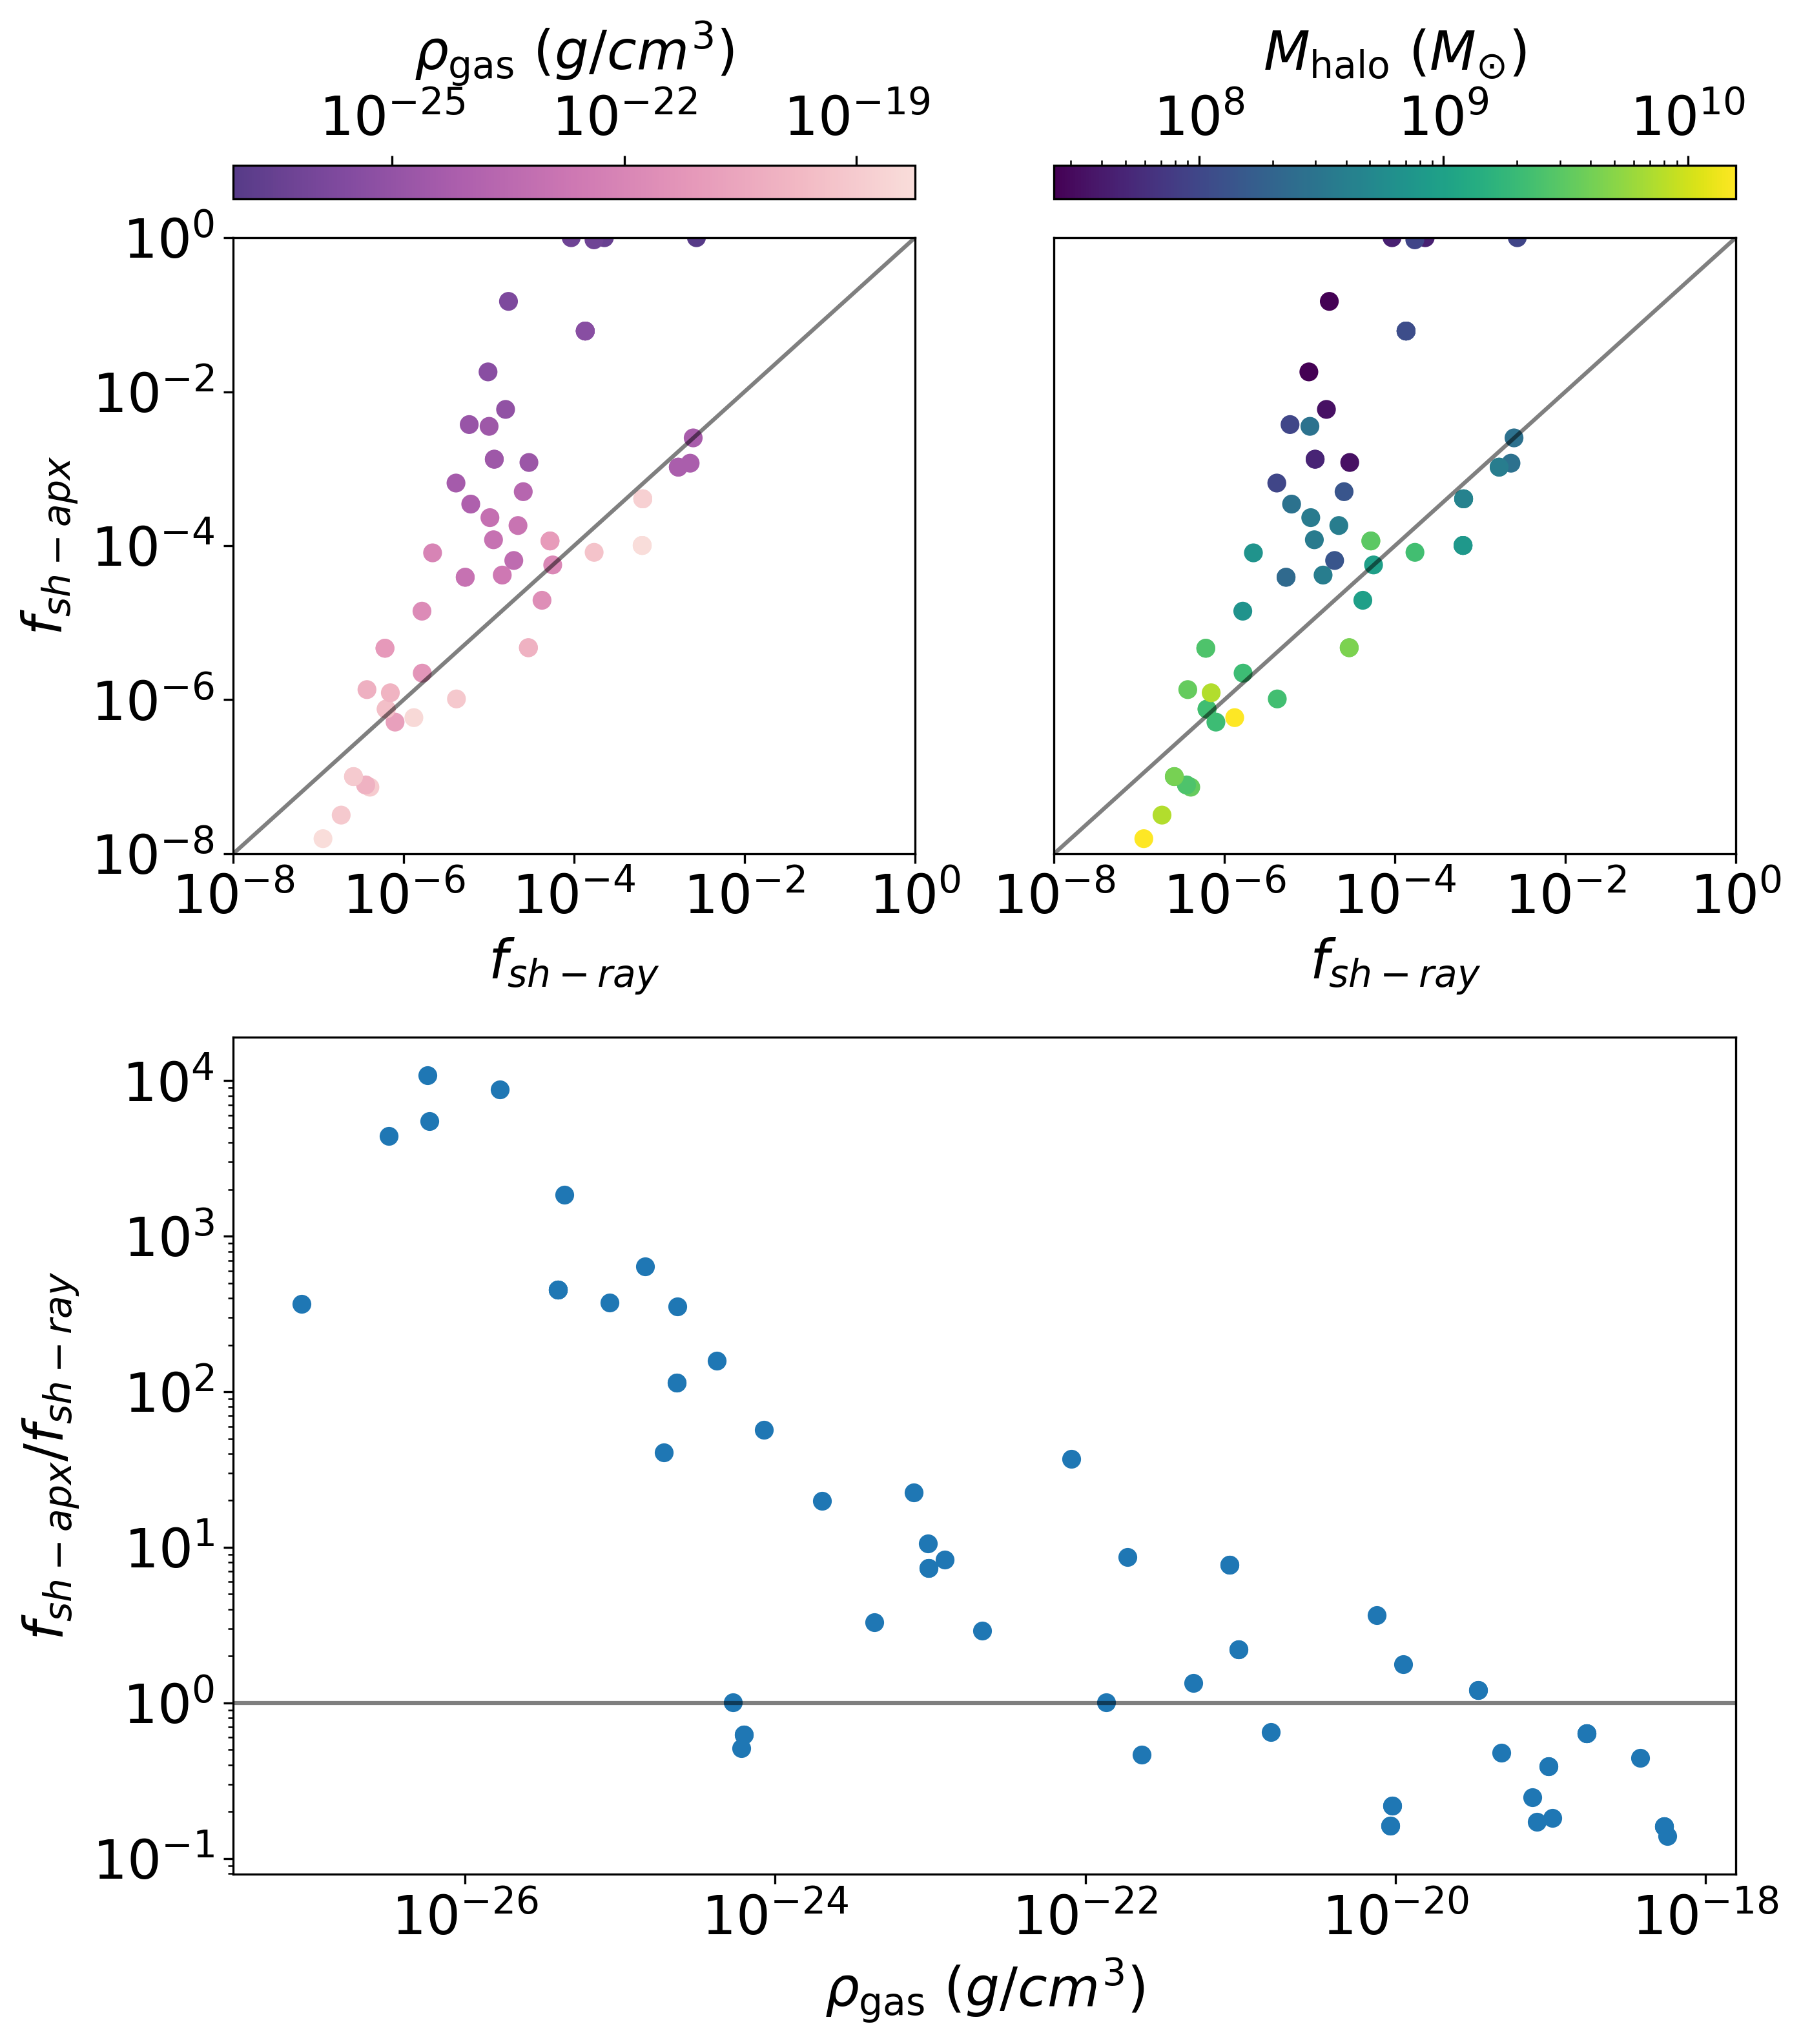
\includegraphics[width=0.95\columnwidth]{EarlyRe/fsh_comparison_ver2.png}
	\caption{The comparison between the self-shielding factor between the \textit{EarlyRe-ray} and the \textit{EarlyRe-apx} simulation, evaluated at $z$ = 10.9. Two gas cells with the highest gas density and highest gas density gradients are chosen in 31 halos in different mass range to evaluate the self-shielding factors. (Top) The relationship between the self-shielding factors calculated by the Sobolev-like approximation model and the ray-tracing model, colored by the cell's gas density (top left) and the host halo's mass (top right). (Bottom) The ratio between the approximated and the ray-traced self-shielding factors is plotted as a function of gas density. The Sobolev-like approximation tends to overestimate the amount of $H_{2}$ self-shielding in the high gas density regime and underestimate it in the low gas density regime.}
	\label{fig:fsh_comparison}
\end{figure}

Figure~\ref{fig:fsh_comparison} compares the self-shielding factor $f_{sh}$ between the ray-tracing model and the Sobolev-like approximation model. At the time step corresponding to z = 10.9, we select 31 halos that contain stars or overlap with another halo that contains stars. For each halo, we select two gas cells to evaluate the self-shielding factor: (1) the gas cell with the highest gas density, and (2) the gas cell with the highest gas density gradient. Each scatter point in Figure~\ref{fig:fsh_comparison} represents a selected gas cell. In the approximation model, the self-shielding factor of a gas cell is calculated using Equations~\ref{eq:self_shielding_factor_eq} and \ref{eq:NH2_approximation}. For the ray-tracing model, since the simulation output does not store the photodissociation rate calculation, we need to re-compute the self-shieling factor using Equation~\ref{eq:self_shielding_factor_eq} with an attenuated LW flux-weighted average column density. The LW flux from each star to a selected gas cell is calculated as follows. Firstly, the intrinsic spectrum of a star particle is generated using the Flexible Stellar Population Synthesis (fsps) with the age and metallicity of the star particle as inputs. We assume an initial mass function from \cite{Dave+2008} evaluated at z = 0, and we use the MIST isochrone library and MILES spectral library to generate the spectra. \textbf{may cite Susie's paper here or ask her for more information}. Then, we calculate the attenuation by including both scattering and absorption due to H/He and metals \textbf{Ask Kirk to include how the absorption and scatterings are computed}. With the scattering and absorption coefficients, we can compute the total optical depth and then the attenuation of the stellar spectrum from the source to the target gas cell. Lastly, we calculate the attenuated flux of each source to the gas cell, compute the LW flux-weighted average $H_{2}$ column density, and get the self-shielding factor from the ray-tracing model. It is important to note that we only include stars within the halo's virial radius to estimate the flux-weighted average $H_{2}$ density because stars outside the radius are too far from the selected gas cell to contribute considerably to the total flux at the selected gas cell. 

Figure~\ref{fig:fsh_comparison} demonstrates a clear disparity in the $f_{sh}$ value between EarlyRe-apx and EarlyRe-ray. In particular, the approximation model tends to overestimate the amount of shielding for cells with a gas density larger than $10^{-20} g/cm^3$ by up to 1 dex. On the other hand, diffuse gas is subjected to underestimated $H_{2}$ self-shielding when the Sobolev-like approximation model is used. For highly diffuse gas, this underestimation can be up to 3-4 dex. This connection between gas density and $f_{sh}$ implies a mass-dependent effect of the self-shielding approximation model on halos. The top right subfigure of Figure~\ref{fig:fsh_comparison} shows that larger halos ($M_{\text{halo}} > 10^{9.5} M_{\odot}$) have their molecular cloud region over-shielded in the approximation model because the gas is denser. On the other hand, the molecular clouds in small halos ($M_{\text{halo}} < 10^{8.5} M_{\odot}$) are under-shielded against LW radiation when using the Sobolev-like approximation. In some cases, the approximation returns no shielding effect even though those gas cells are still weakly shielded ($f_{sh} \approx 10^{-3}$ when ray-tracing is utilized. Only molecular gas clouds in halos whose mass is about $10_{9} M_\odot$ are well modeled in the approximation model. The significance of this effect on star formation will be explored in Section~\ref{subsect:effect_on_sf}.

\textbf{Maybe a comparison in terms of the time run between the two methods}

\subsection{Cross-matching halos}
\label{subsect:cross-matching_halos}
To examine how each individual halo is affected by the implementation scheme of $H_{2}$ self-shielding, we perform cross-matching between halos in the simulations with ray-tracing (\textit{EarlyRe-ray} and \textit{LateRe-ray} sets) and their counterparts in the simulations with the Sobelev-like approximation (\textit{EarlyRe-apx} and \textit{LateRe-apx} sets). The matching requirements are
\begin{align}
    & \frac{2}{3} < \frac{M_{vir_{ray}}}{M_{vir_{apx}}} < \frac{3}{2} \nonumber \\
    \frac{d_{\text{COM}}}{R_{vir_{ray}}} & < 0.25 \; , \; \frac{d_{\text{COM}}}{R_{vir_{apx}}} < 0.25 
\label{eq:crossmatching_requirement}
\end{align}
The virial mass and radius in Equation~\ref{eq:crossmatching_requirement} come from ROCKSTAR and are calculated using only dark matter. We cross-match all the halos at the last timestep of the simulations and then trace back their merger tree using the \texttt{consistent-tree} outputs (details in Subsection~\ref{sec:halotracking}).

\subsection{Star assignment}
\label{subsect:star_assignment}

We uniquely assign each star particle in the simulation to one dark matter halo in a two-step fashion. For the first step, a star particle is assigned to a halo where it is first created. If a star particle is created inside the intersection of multiple halos, we will calculate the orbital energy of that star particle with respect to each halo's center to determine which halo the particle belongs to. The assigned halo is the one with lower relative total orbital energy. We assume that a star particle never leaves its assigned halo unless that halo merges with another one, in which case the star particle will become a member of the descendant halo of the merger. This assumption allows a quick assignment of stars to halos without the need to calculate the orbital energy of each star to multiple halos, which is computationally expensive. The assignment's first step starts from the first snapshot to the last snapshot of the simulation. 

Even though stars do not generally leave a halo's potential well for isolated halos, the behavior becomes more complex during halo-halo interaction as stripping can occur and stars can be lost from one halo to another \citep{Kannan+2015}. Therefore, the second step of our process is to address this shortcoming of the first step's assumption and to refine the star assignment result. In this step, we validate the output from the first step and check whether a star remains in its assigned halo's virial radius throughout its lifetime. If a star escapes the virial radius of its originally assigned halo, we assign that star to a new halo under two conditions: (1) the star's position must be within the new halo's virial radius and (2) the star's total orbital energy with respect to the new halo must be negative. Similar to the first step, if a star is located inside multiple potential new halos, we assign that star to the halo with the lowest negative orbital energy. If either Condition (1) or (2) fails at a certain timestep, this suggests that the star is stripped out of the potential well of all halos and thus we remove that star from the halo assignment process of that time step. 

Once each star particle is uniquely associated with one halo, we calculate a halo's stellar mass and SFR exclusively based on its member star particles. This gravitational unbinding of star particles guarantees that each halo's stellar mass profile are not overlap and independent of each other. 

\subsection{Defining ISM, CGM, and IGM}

The boundary of the interstellar medium (ISM), the circumgalactic medium (CGM), and the intergalatic medium (IGM) region in our analysis is defined as follows. The ISM region (or the boundary of a galaxy) starts from the galaxy's center of mass to $R_{\mathrm{bary}, 2000}$, which is the radius enclosing a baryonic (gas and stars) mass density 2000 times the universe's critical mass density at a certain redshift. Even though there are multiple other definition of the boundary of galaxy in literature, such as using a fixed fraction of the virial radius, a fixed physical radius, or a radius that is scaled with mass or surface brightness (see \citealp{Stevens+2014} for a summary of these techniques), our over-density approach helps define the galaxy more robustly and more physically because it is redshift and density dependent. It also helps better define the galaxy during a close galaxy interaction when a half-mass radius or half-light radius approach may fail as another galaxy is in the target galaxy's virial radius. Depending on the redshift and the galaxy's compactness, $R_{\mathrm{bary}, 2000}$ typically ranges from 0.15 to 0.25 times the halo's virial radius, which falls in the same range as other galaxy's aperture definitions in cosmological simulations \citep{Stevens+2014}. The CGM starts from $R_{\mathrm{bary}, 2000}$ to $R_{\mathrm{halo,vir}}$, and the IGM is the region outside of the virial radius of all halos.

Also, it is important to note that the baryonic center of mass does not always coincide with the halo's center of mass. Thus, in some cases, we shift the virial region to be centered on the gas and stellar mass instead of the dark matter mass; however, this shift is not large and does not affect our interpretation.    
 
\section{Results}

\subsection{Effect on the molecular hydrogen content and star formation}
\label{subsect:effect_on_sf}

\begin{figure}[h]
    \centering
    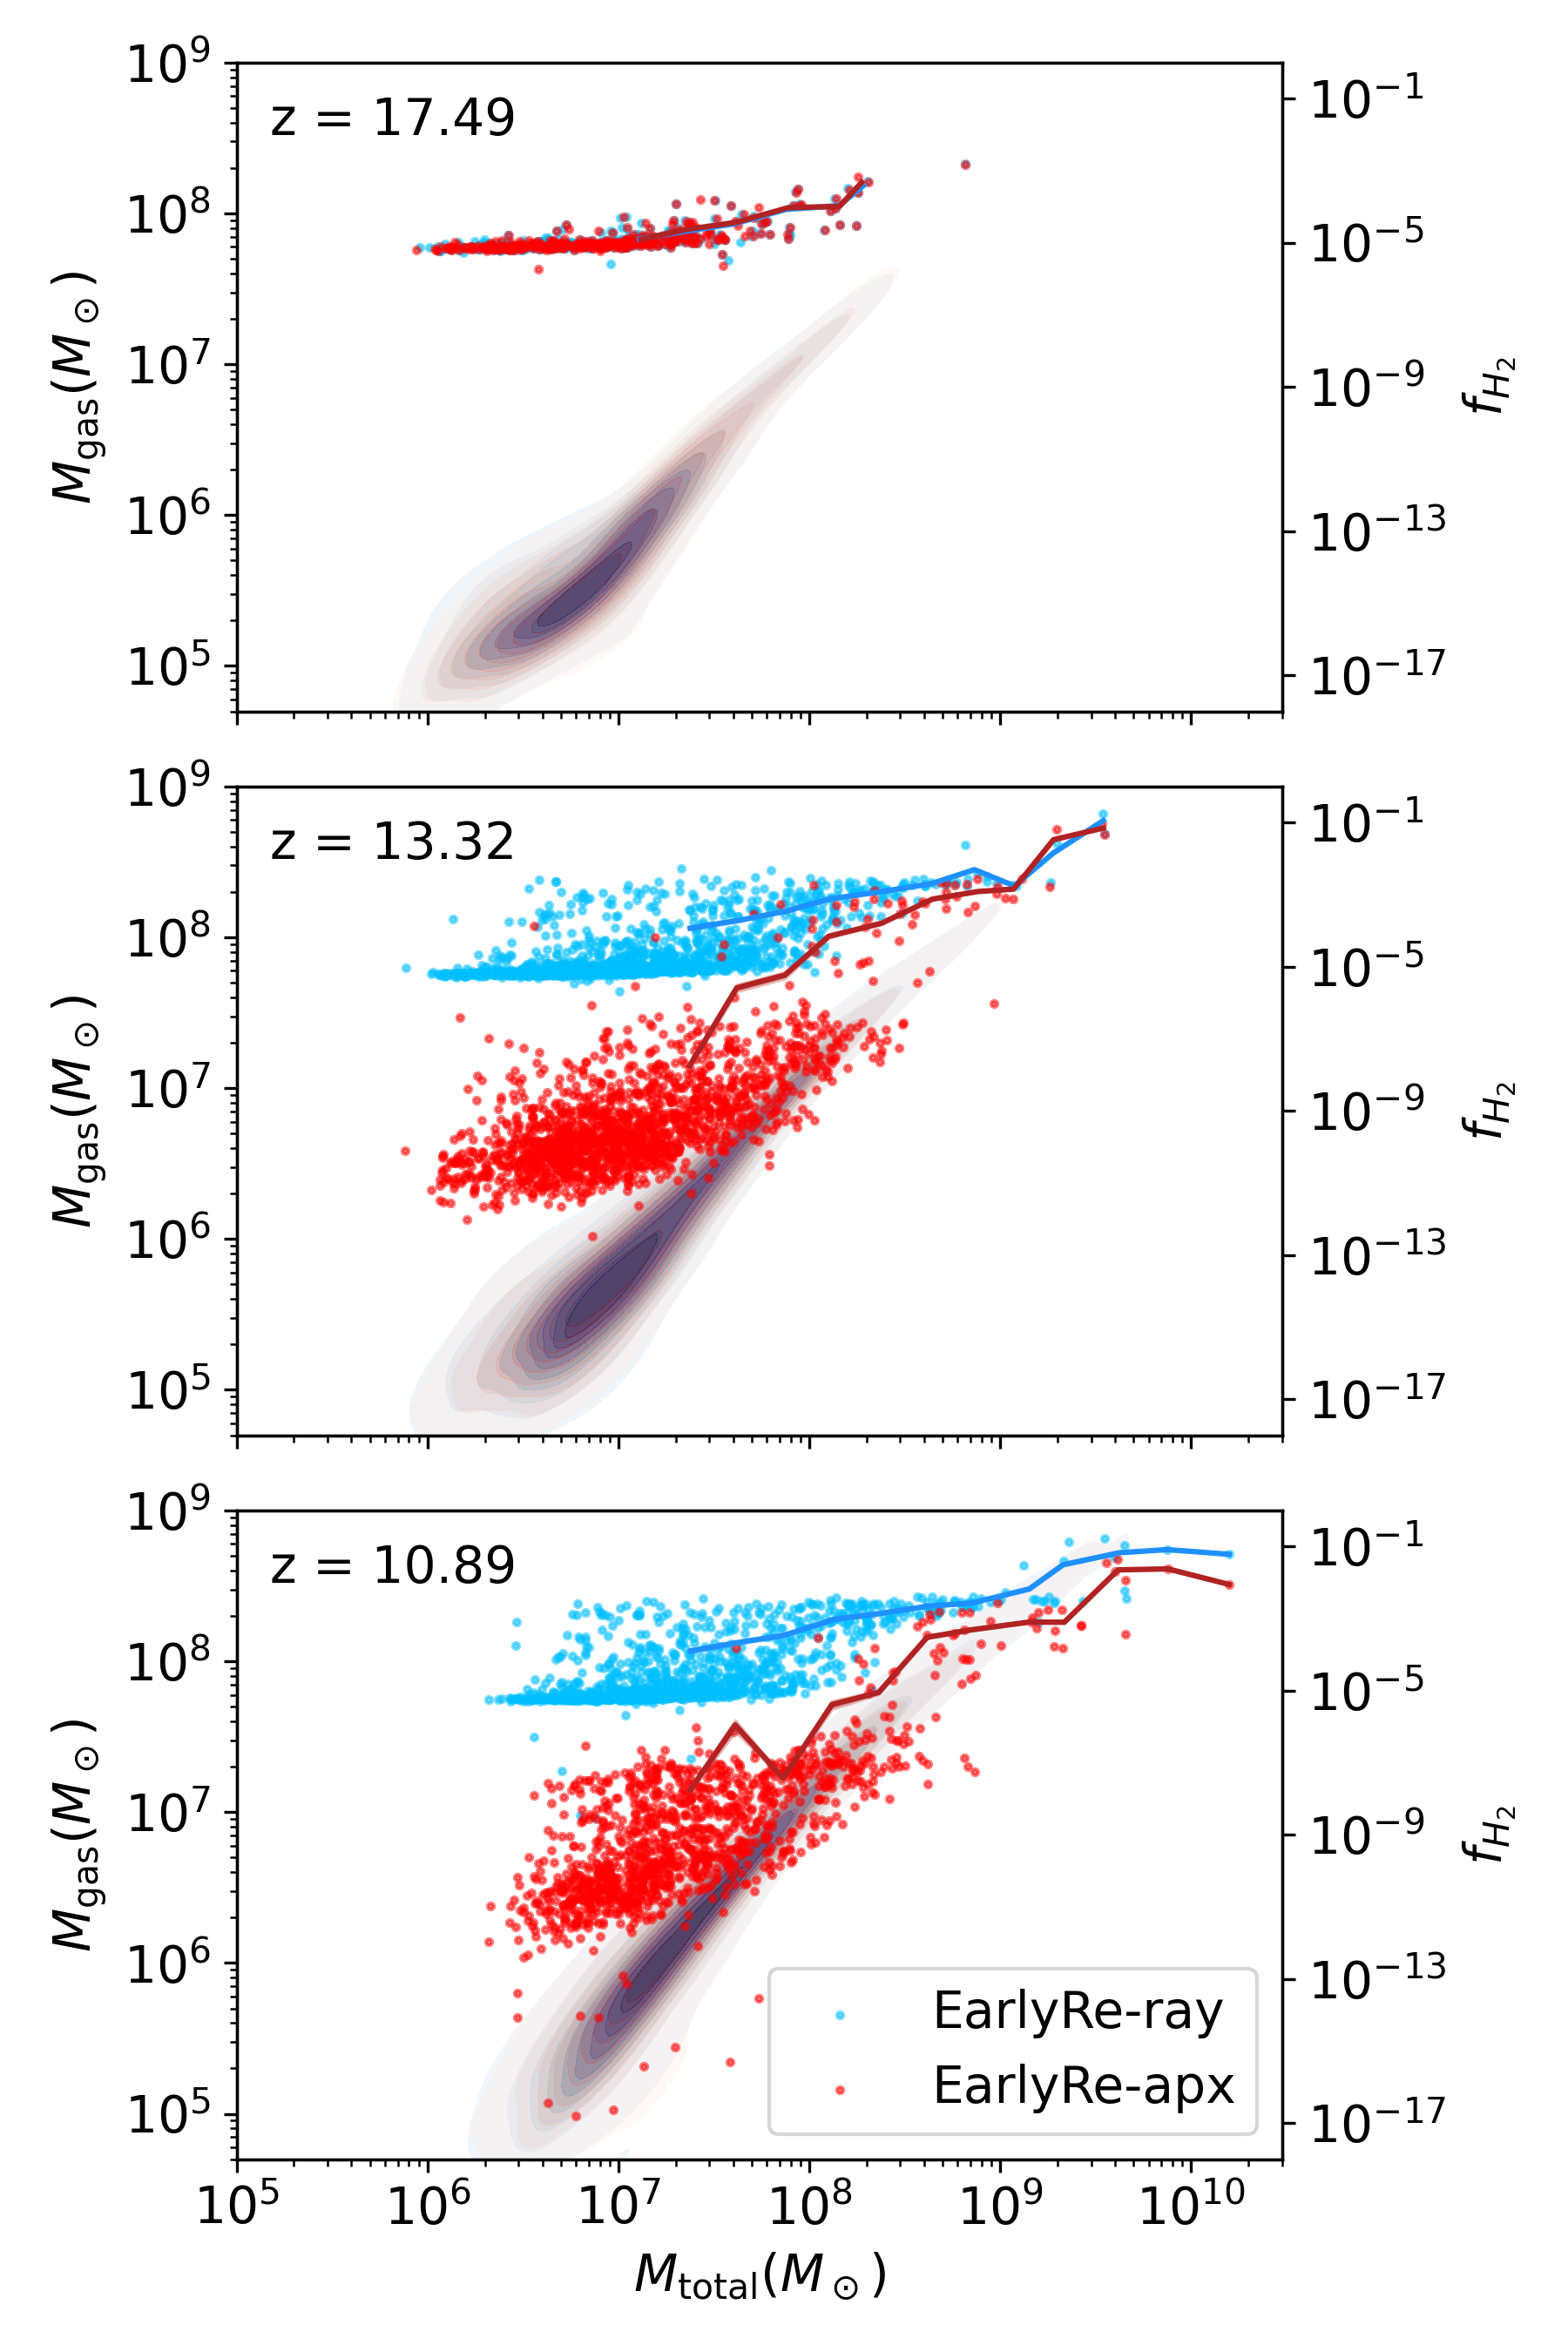
\includegraphics[width=0.9\columnwidth]{EarlyRe/h2_frac_gasmass_distribution_EarlyRe_shinbad.png}
    \caption{The relationship between the $H_{2}$ fraction and the total mass in the timestep where stars first appear, in the intermediate, and in the last timestep of the \textit{EarlyRe} dataset. The contour plots show the $M_{\text{gas}}$ distribution and the scatter points show the $H_{2}$ fraction of all halos in the simulation box.}
    \label{fig:H2_frac_EarlyRe}
\end{figure}

Because the column density approximation model directly concerns the calculation of the molecular hydrogen density, we first investigate the amount of $H_{2}$ in the ray tracing and approximation treatment. Figure~\ref{fig:H2_frac_EarlyRe} shows the $H_{2}$ fraction ($f_{H_{2}}$), which is the ratio between the $H_{2}$ mass with the total gas mass, as a function of the total halo mass in three snapshots, one at the time where star particles first appear in the simulations (z $\approx$ 17.49), one at the time step in the middle of the simulation run (z $\approx$ 13.32), and one being the last time step of the run (z $\approx$ 10.9). Each halo in the snapshot is represented by a scatter point, the line represents the running average of each total mass bin, and the shaded region around the line is the standard deviation of the scatter points within each mass bin. The contour plots represent the distribution of the halos in the $M_{\text{gas}} - M_{\text{total}}$ space. According to Figure~\ref{fig:H2_frac_EarlyRe}, both EarlyRe-ray and Early-apx simulations have similar gas mass distribution across all timesteps, showing $f_{H_{2}}$ represents the amount of $H_{2}$ in the halos. However, $f_{H_{2}}$ shows a notable difference between the two radiative transfer treatments, especially at the later time step and in the lower-halo-mass regime. For halo mass smaller than $10^{8} M_\odot$, the $f_{H_{2}}$ in the ray-tracing treatment is larger than that of the Sobolev-like approximation treatment by 3 to 6 dex. This difference grows larger as the simulation evolves, reaching up to 12 dex at the last time step for small halos. The EarlyRe-ray simulation also develops a lower limit for $f_{H_{2}}$ of around $10^{-5}$, whereas the $f_{H_{2}}$ is allowed to reach much further value in the EarlyRe-apx simulation. This shows that the ray-tracing treatment models the self-shielding effect much better and thus helps preserve more molecular hydrogen in the halos. As pointed out in Figure~\ref{fig:fsh_comparison}, the approximation treatment considerably underestimates $H_{2}$ self-shielding in a low gas density regime and molecular hydrogen to get photodissociated more easily, inferring that smaller halos are the most susceptible to the choice of the model. At a higher mass range, the difference in $f_{H_{2}}$ between the two models gradually diminishes. This is reasonable because larger halos have deeper gravitational potential well and have more dense cool gas regions where $H_{2}$ exists. In these regions, the approximation model matches well with the ray-tracing model (as shown in Figure~\ref{fig:fsh_comparison}), leading to an agreement of $f_{H_{2}}$ between the two runs. 

\begin{figure*}
    \centering
    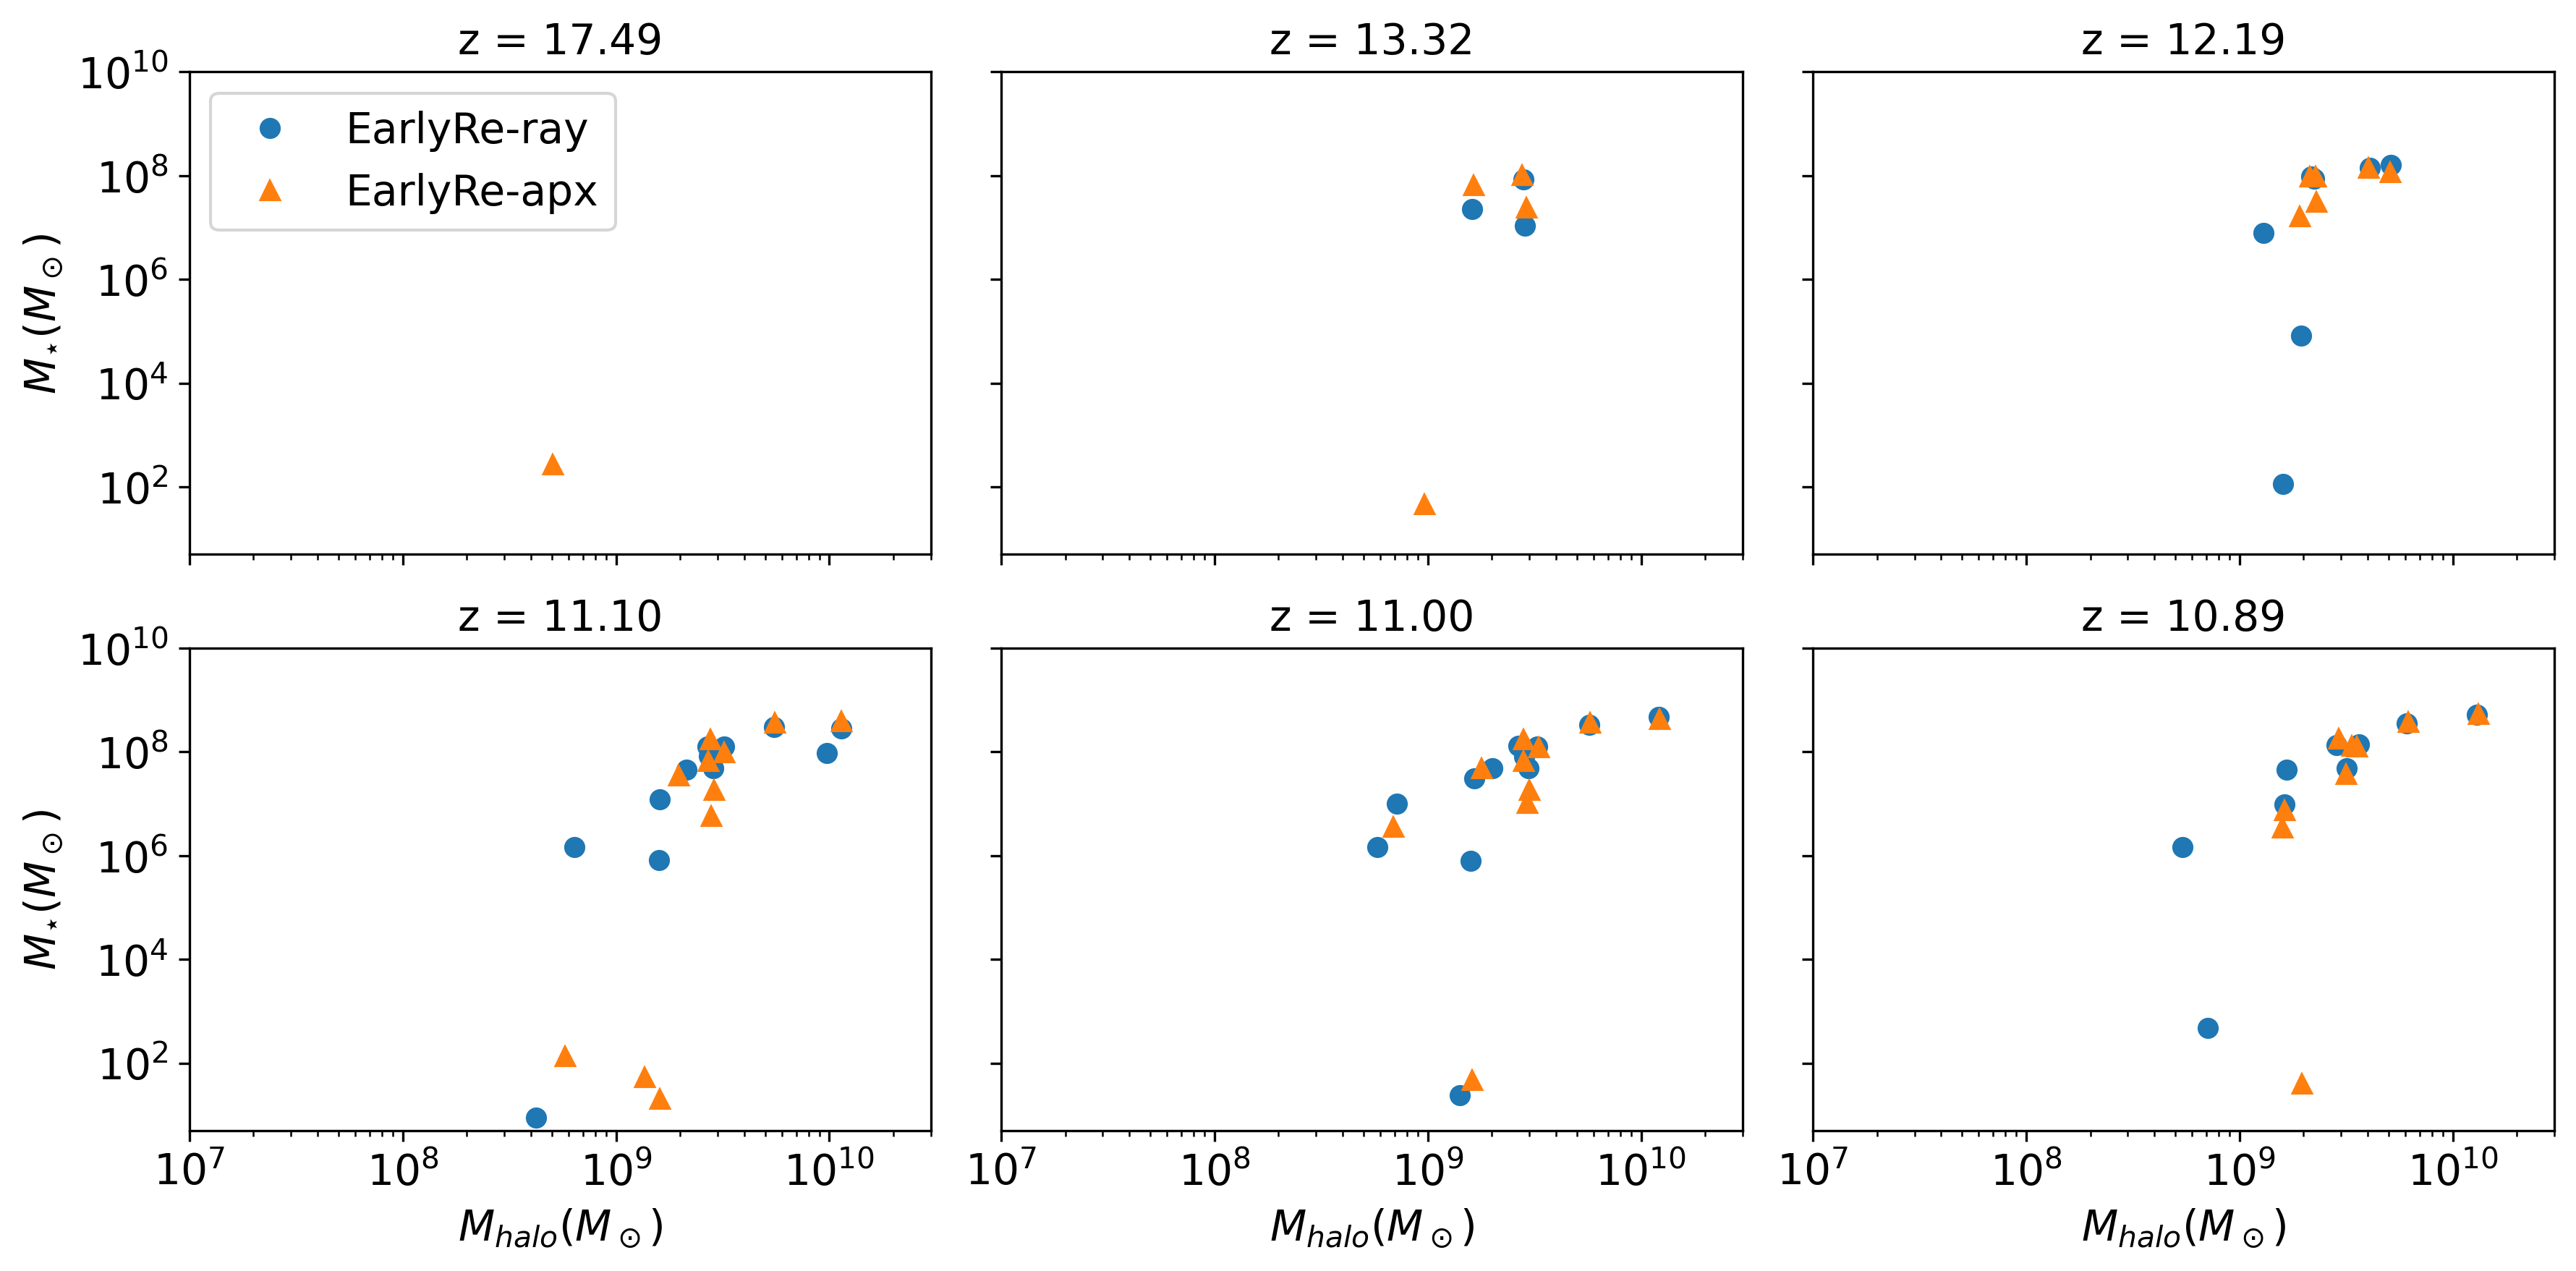
\includegraphics[width=0.95\textwidth]{EarlyRe/stellarmass_totalmass_EarlyRe_starassignment.png}
    \caption{The relationships between stellar mass and total mass of all the halos in the timestep where stars first appear, in the intermediate timesteps, and in the last timestep of the \textit{EarlyRe} dataset.}
    \label{fig:SFR_stellar_total_EarlyRe}
\end{figure*}
\begin{figure}
    \centering
    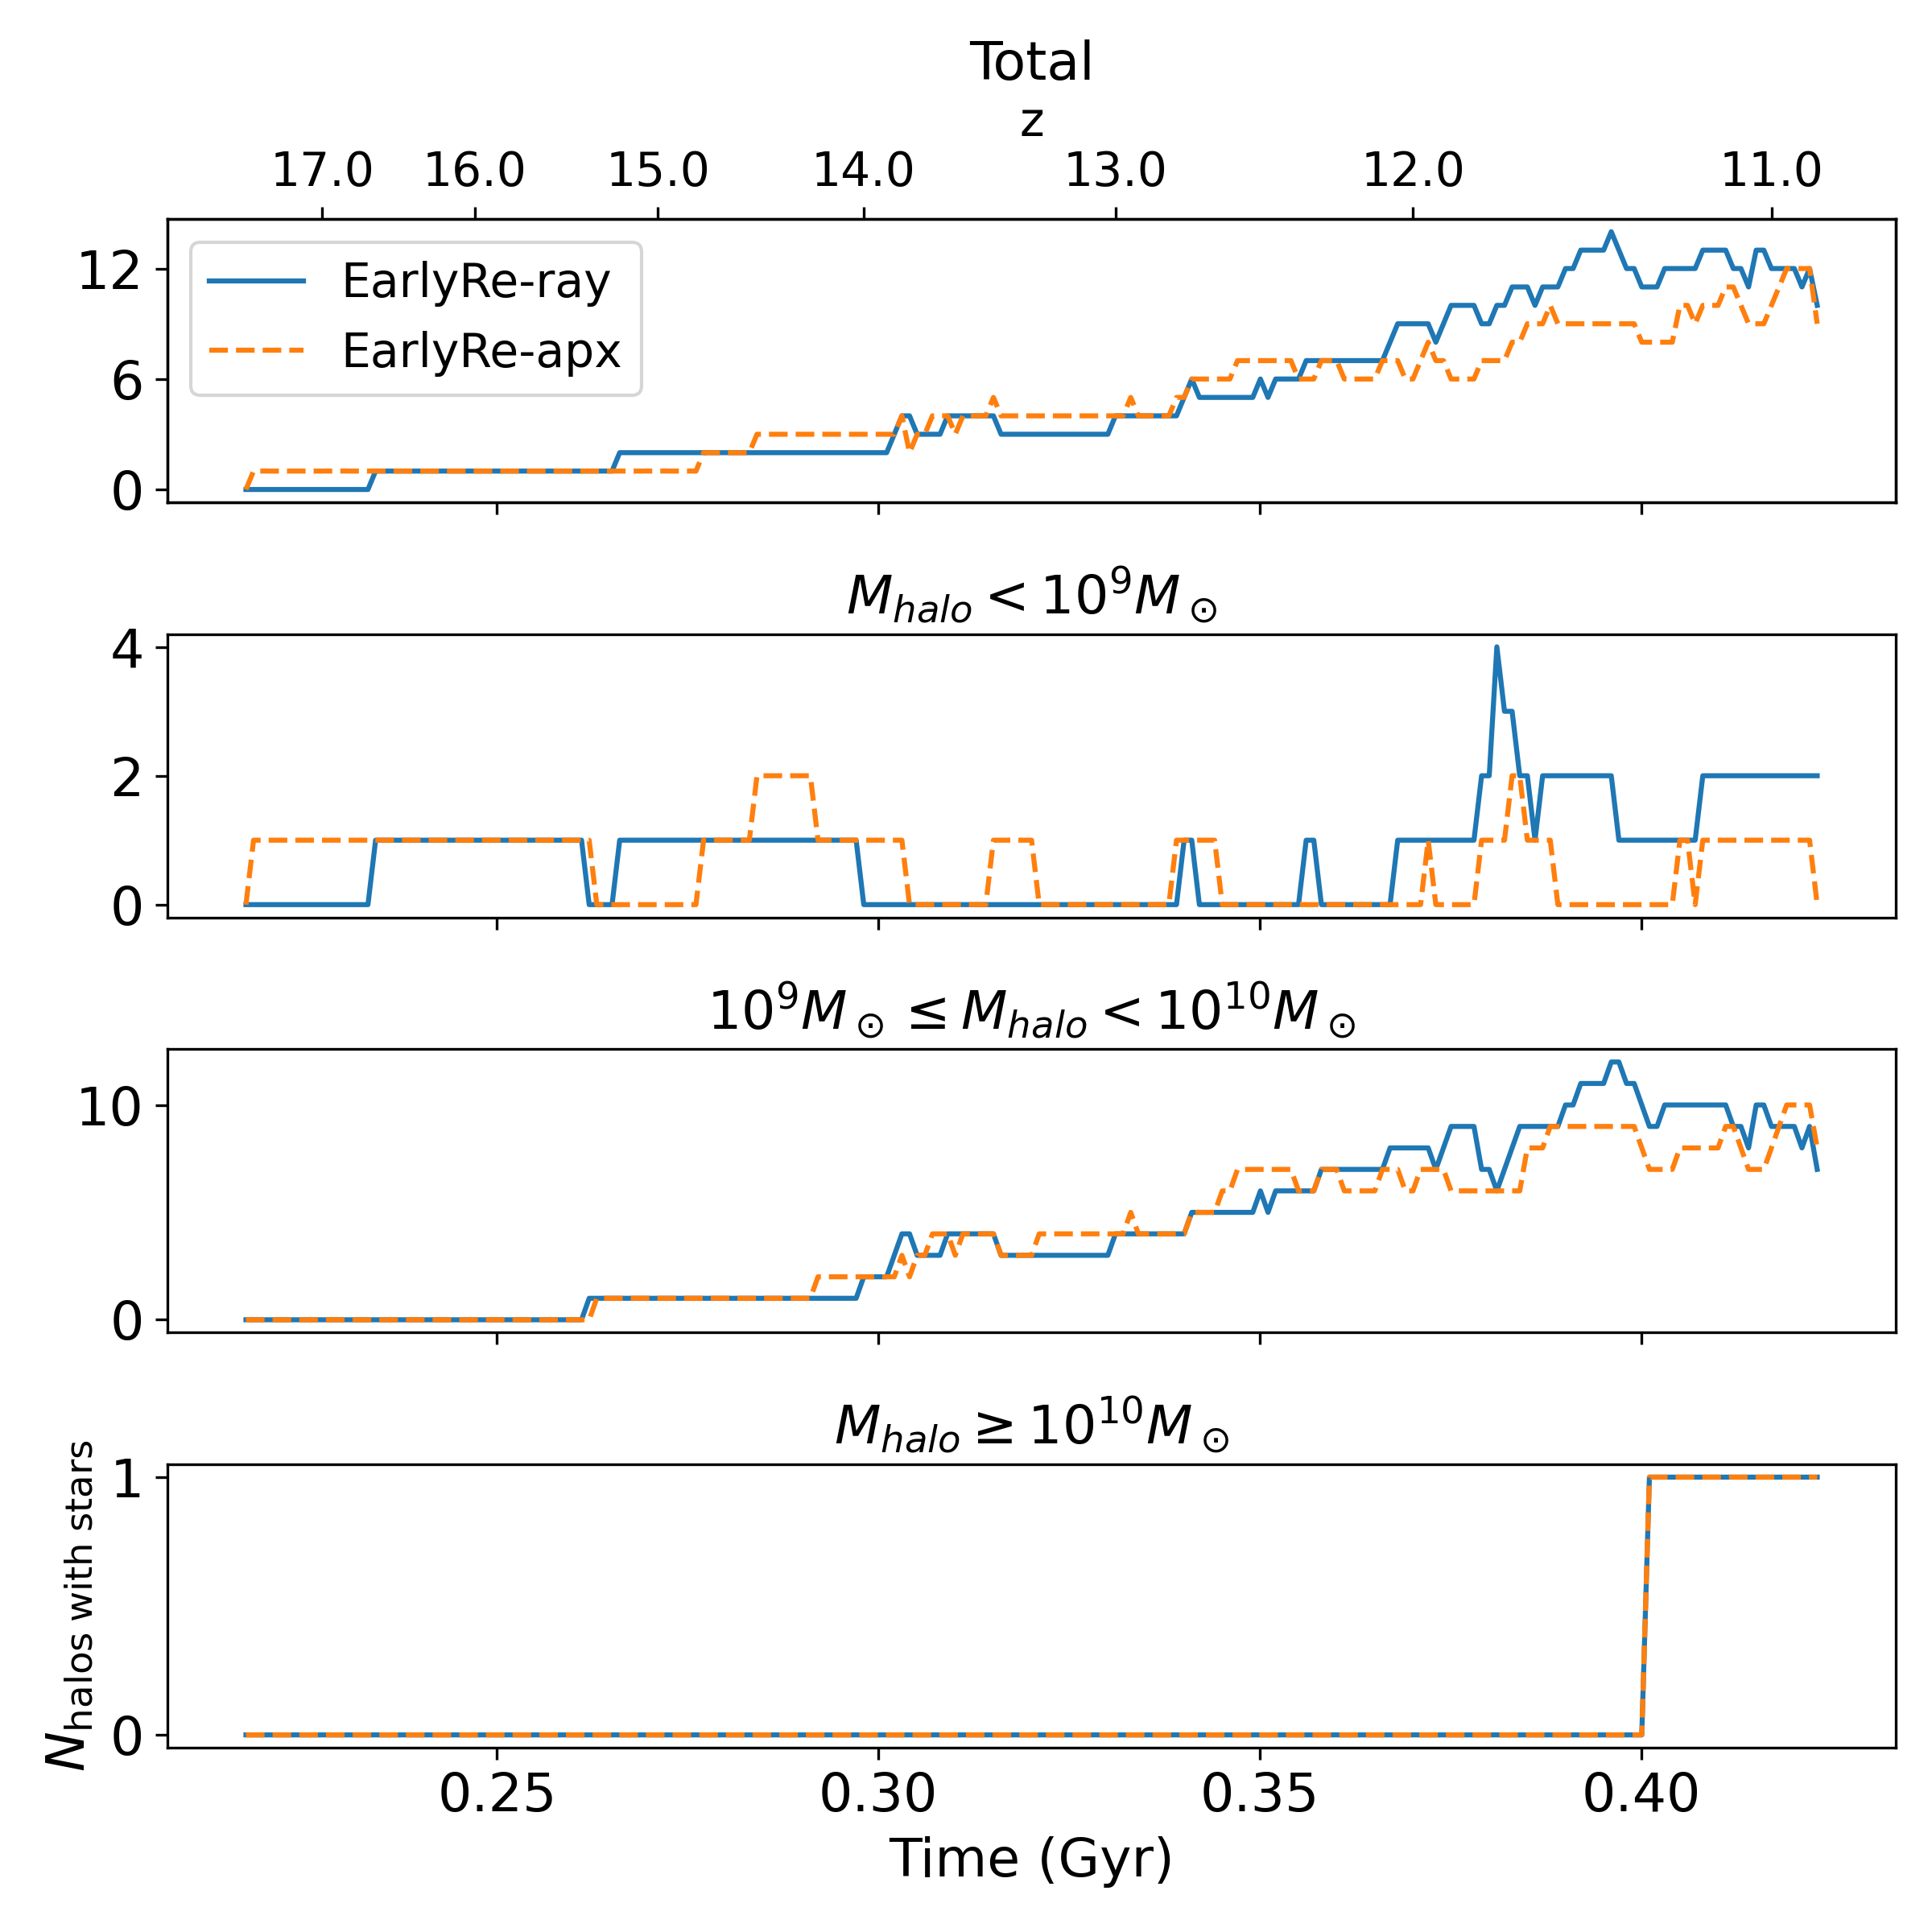
\includegraphics[width=0.95\columnwidth]{EarlyRe/number_of_halo_wstars.png}
    \caption{The comparison between the number of halos with stars as a function of time for each halo mass bin between the \textit{EarlyRe-ray} and the \textit{EarlyRe-apx} simulations.}
    \label{fig:number_halowstars_vs_time_EarlyRe}
\end{figure}


We proceed to investigate whether the self-shielding treatment affects the stellar mass of galaxies in the simulation. Figure~\ref{fig:SFR_stellar_total_EarlyRe} shows the relationship between stellar mass and halo mass between the \textit{Early-Ray} and \textit{Early-apx} in the time step where stars first appear (top left panel), in the last time step of the dataset (bottom right panel), and in the intermediate time steps. Figure~\ref{fig:number_halowstars_vs_time_EarlyRe} displays the number of halos that host stars as a function of time for different halo mass bins. The stellar component of the halos is unbinded by using the star assignment procedure described in Section~\ref{subsect:star_assignment}. Even though the number of halos with stars is even between \textit{EarlyRe-apx} and \textit{EarlyRe-ray} in the beginning, there are more halos with stars in \textit{EarlyRe-ray} at the end of the simulation, particularly halos with $M_{halo} < 10^{9} M_\odot$. For ease of reference and lack of a better term, we will use the term "galaxy" to refer to a halo with stars, as opposed with halos with only gas and dark matter particles. From 375 million years after the Big Bang to near the end of the simulation ($z \approx 11.88 - 11$), there are two to four galaxies more in the simulation with the ray-tracing treatment. Furthermore, at a similar halo mass, smaller halos in \textit{EarlyRe-ray} tend to have more stars than their counterparts in \textit{EarlyRe-ray} by several dex in solar mass. This indicates that the use of Sobolev-like approximation for $H_{2}$ self-shielding treatment inhibits star formation activity in small halos and dwarf galaxies. On the other hand, halos whose dark matter mass is larger than $10^{9} M_\odot$ show good agreement in stellar mass, suggesting that the stellar components of large halos are unaffected by our choice of $H_{2}$ self-shielding model. This observation aligns with Figure~\ref{fig:H2_frac_EarlyRe}, where we see that $H_{2}$ is more accurately shielded in higher halo mass in \textit{EarlyRe-apx}.

Another difference between \textit{EarlyRe-ray} and \textit{EarlyRe-apx} is the time when star particles first appear in the simulation. According to Figure~\ref{fig:number_halowstars_vs_time_EarlyRe}, the formation of the first galaxy in \textit{EarlyRe-apx} occurs 16 million years before that in \textit{EarlyRe-ray}. The first galaxies in the two simulations both form in a halo with a dark matter mass smaller than $10^{9} M_\odot$. This is rather intuitive, given that previous evidence shows that for small halos, stars form easier in the simulation using a ray-tracing model. However, further investigation suggests that the timing disparency in the formation of first stars is likely due to a stochastic nature of our star formation prescription rather than a physical reason. Before the first stars appear in a halo in \textit{EarlyRe-apx}, the temperature and density distribution of gas and molecular hydrogen of the counterpart halo in \textit{EarlyRe-ray} are similar to the halo in \textit{EarlyRe-apx}. More discussion and plots regarding the first galaxies in the two simulation will be directed to the Appendix. \textbf{Reminder to include the appendix}


%To investigate the effect of the $H_{2}$ self-shielding radiative transfer treatment on individual halos, we identify 9 matching halos with stars between \textit{EarlyRe-ray} and \textit{EarlyRe-apx} using the method listed in Section~\ref{subsect:cross-matching_halos}. Figure~\ref{fig:H2_phase_plot_Branch-0_EarlyRe} shows the temperature-density phase plot of molecular hydrogen in the largest halo (Branch~0) at the last snapshot of the simulation. The dashed vertical line denotes the implemented star formation threshold density $n_{H,\text{thres}} = 1\;\text{cm}^{-3}$ (\textbf{confirm again}) or $\rho_{H_{2},\text{thres}} = 3.35\times10^{-24}\;\text{g}\,\text{cm}^{-3}$. The difference in $H_{2}$ behavior is evident between the two subplots. In \textit{EarlyRe-ray}, molecular hydrogen gas can cool down to $\approx 40$ K and form denser clouds that surpass the star formation density threshold. These cool dense clouds also account for most of the $H_{2}$ mass in the halo, inferring a great potential to form stars in the halo. On the other hand, the counterpart halo in the \textit{EarlyRe-apx} has much less molecular hydrogen reservoir. Specifically, even though their total gas mass is equivalent ($\approx 2\times10^{9}\;M_\odot$), Halo Branch 0 of \textit{EarlyRe-ray} has 7 times more $H_{2}$ compared to \textit{EarlyRe-apx}. \textbf{Keep writing, explain the vertical downward line in EarlyRe-apx (cool less-dense gas). Also, investigate while the gas mass is larger in the ray scheme, the stellar mass between the two simulations are the same -> More stars created, more feedback that prevents gas from forming (increase velocity divergence), even though there are more gas available?}.

%This result gives us a more detailed look at the disparity of $H_{2}$ when using the ray-tracing scheme and the Sobolev-like approximation scheme and reaffirm the results from Figure~\ref{fig:H2_frac_EarlyRe}. The other eight matched halo pairs also show a similar pattern. Thus, for brevity, we do not show their phase plots.

\subsection{Case study}

In this section, we analyze the properties of two halos, one being the largest halo in the simulation and one having a halo mass of $X M_\odot$, which is in the mass range where the approximation in $H_{2}$ self-shielding fails to accurately model star formation, as suggested in Figure~\ref{fig:SFR_stellar_total_EarlyRe}. We match the halos between \textit{EarlyRe-ray} and \textit{EarlyRe-apx} using the procedure in Section~\ref{subsect:cross-matching_halos}. These two pairs of halos serve as examples to how the $H_{2}$ self-shielding modeling affects the galaxy properties. 

\begin{figure*}
	\gridline{\fig{EarlyRe/Halo0-0_property_comparison_Snapshot_211_Projection_x_ver1088.png}{0.375\textwidth}{}
		\fig{EarlyRe/Halo0-0_property_evolution_comparison_ver1088.png}{0.615\textwidth}{}}
	\caption{(Left) The gas density, $H_{2}$ density, temperature, metallicity, and stellar surface density projection plot of Halo 0 ($M_{\mathrm{halo}} \approx 1.3\times 10^{10} M_\odot$ at z = 10.89) within one virial radius. The white circle represents the boundary of the galaxy, which is defined as the radius enclosing the baryonic density 2000 times larger than the critical density of the universe. (Right) The time evolution of different properties in Halo 0 between the \textit{EarlyRe-ray} and \textit{EarlyRe-apx} simulations.}
	\label{fig:Halo0-0_comparison}
\end{figure*}

\begin{figure*}
	\gridline{\fig{EarlyRe/Halo8-9_property_comparison_Snapshot_211_Projection_x_ver1088.png}{0.375\textwidth}{}
		\fig{EarlyRe/Halo8-9_property_evolution_comparison_ver1088.png}{0.615\textwidth}{}}
	\caption{Same as Figure~\ref{fig:Halo0-0_comparison}, but for another halo whose $M_{\mathrm{halo}} \approx 1.7\times 10^{9} M_\odot$ at z = 10.89.}
	\label{fig:Halo8-9_comparison}
\end{figure*}


\subsection{Effect on the ISM and CGM}

Sub-section~\ref{subsect:effect_on_sf} explores how two treatments of modeling $H_{2}$ affect star formation in a halo as a whole. In this section, we more closely examine the effect of $H_{2}$ self-shielding modeling on the ISM, the CGM, and the IGM to help further explain the previous observations we have on star formation. 


\textbf{Make a big figure showing all the halo pairs projection plot at the last snapshot.}

\textbf{Remember to comment on the stellar mass of the galaxies in Figure 5 and 6.}

\begin{figure*}
    \gridline{\fig{EarlyRe/Galaxy_CGM_phaseplot_Halos_0-0_Snapshot_211_ver1088.png}{0.47\textwidth}{(a)}
    \fig{EarlyRe/Galaxy_CGM_H2phaseplot_Halos_0-0_Snapshot_211_ver1088.png}{0.485\textwidth}{(b)}}
    \caption{The gas phase plot (Sub-figure (a)) and the molecular hydrogen phase plot (Sub-figure (b)) of the largest halo ($M_{\mathrm{halo}} = 1.3\times10^{10} M_\odot$) in our simulation set, evaluated at the last time step $z = 10.89$. For each sub-figure, the left column shows the halo in \textit{EarlyRe-apx}, and the right column shows its counterpart in \textit{EarlyRe-ray}. The top row in each subfigure shows the phase plot using the gas cells within the galaxy region ($r \leq R_{bary,2000}$), and the bottom row shows the phase plot using the gas cells in the CGM region ($R_{bary,2000} < r \leq R_{vir}$).} 
    \label{fig:phaseplot_Halo0-0}
\end{figure*}

\begin{figure*}
    \gridline{\fig{EarlyRe/Galaxy_CGM_phaseplot_Halos_18-19_Snapshot_211_ver1088.png}{0.47\textwidth}{(a)}
    \fig{EarlyRe/Galaxy_CGM_H2phaseplot_Halos_18-19_Snapshot_211_ver1088.png}{0.485\textwidth}{(b)}}
    \caption{Similar to Figure~\ref{fig:phaseplot_Halo0-0}, for a halo with mass $M_{\mathrm{halo}} = 7.1\times 10^{8} M_\odot$.}
    \label{fig:phaseplot_Halo18-19}
\end{figure*}


\subsection{Effect on the IGM and reionization}

\begin{figure*}
    \centering
    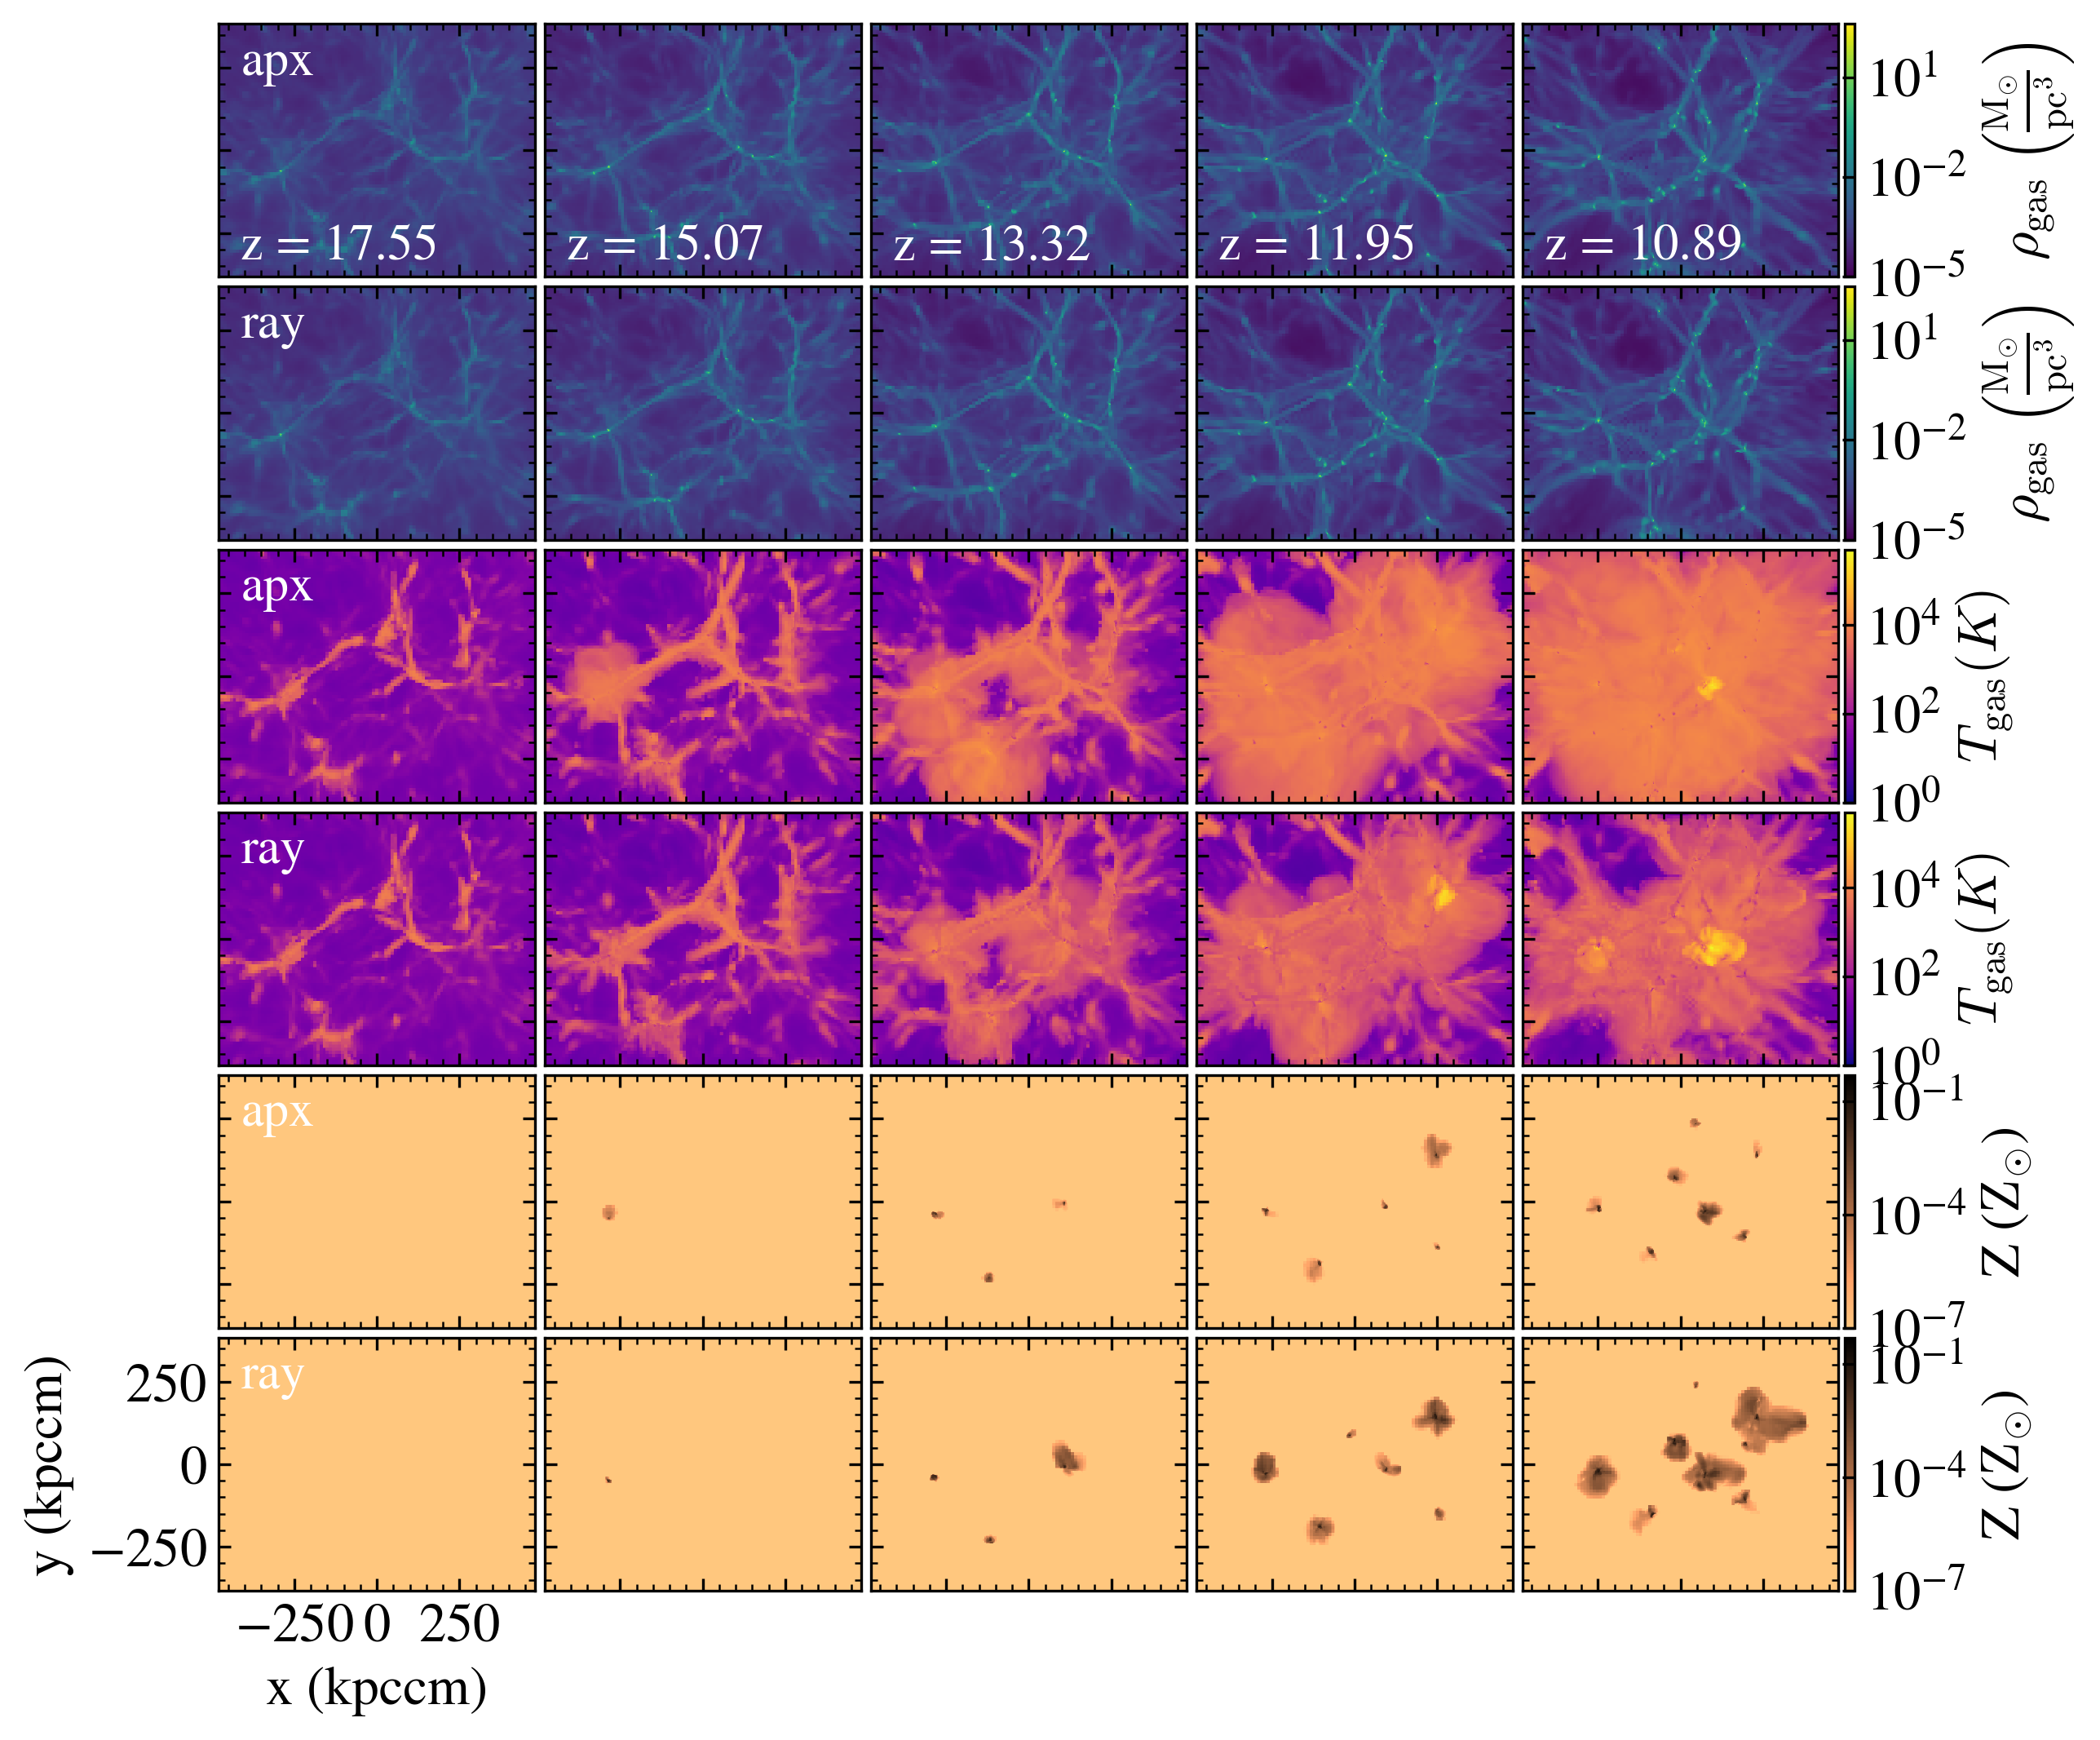
\includegraphics[width=\textwidth]{EarlyRe/gas_surface_density_multiple_ver1088.png}
    \caption{The gas surface density, gas temperature, and gas metallicity within the simulation's refined region between the \textit{EarlyRe-apx} and \textit{EarlyRe-ray}.}
    \label{fig:gas_surface_density_wholebox}
\end{figure*}

\textit{For the radiative star cluster model and the Population III star model used in our simulation, their overdensity thresholds for a star particle to form are $10^{7}$ and $10^{6}$, respectively. At the time step where we evaluate the $f_{sh}$ ($z$ = 10.9), these overdensity thresholds correspond to a gas density threshold of $4.5\times 10^{-20}$ and $4.5\times 10^{-21}$. According to Figure~\ref{fig:fsh_comparison}, these thresholds lie in the regime where $f_{sh}$ is typically over-estimated in the approximation model. On the other hand, $H_{2}$ gas in the interstellar medium (ISM) of \textit{EarlyRe-apx} can be under-shielded.} 



\begin{figure*}
    \centering
    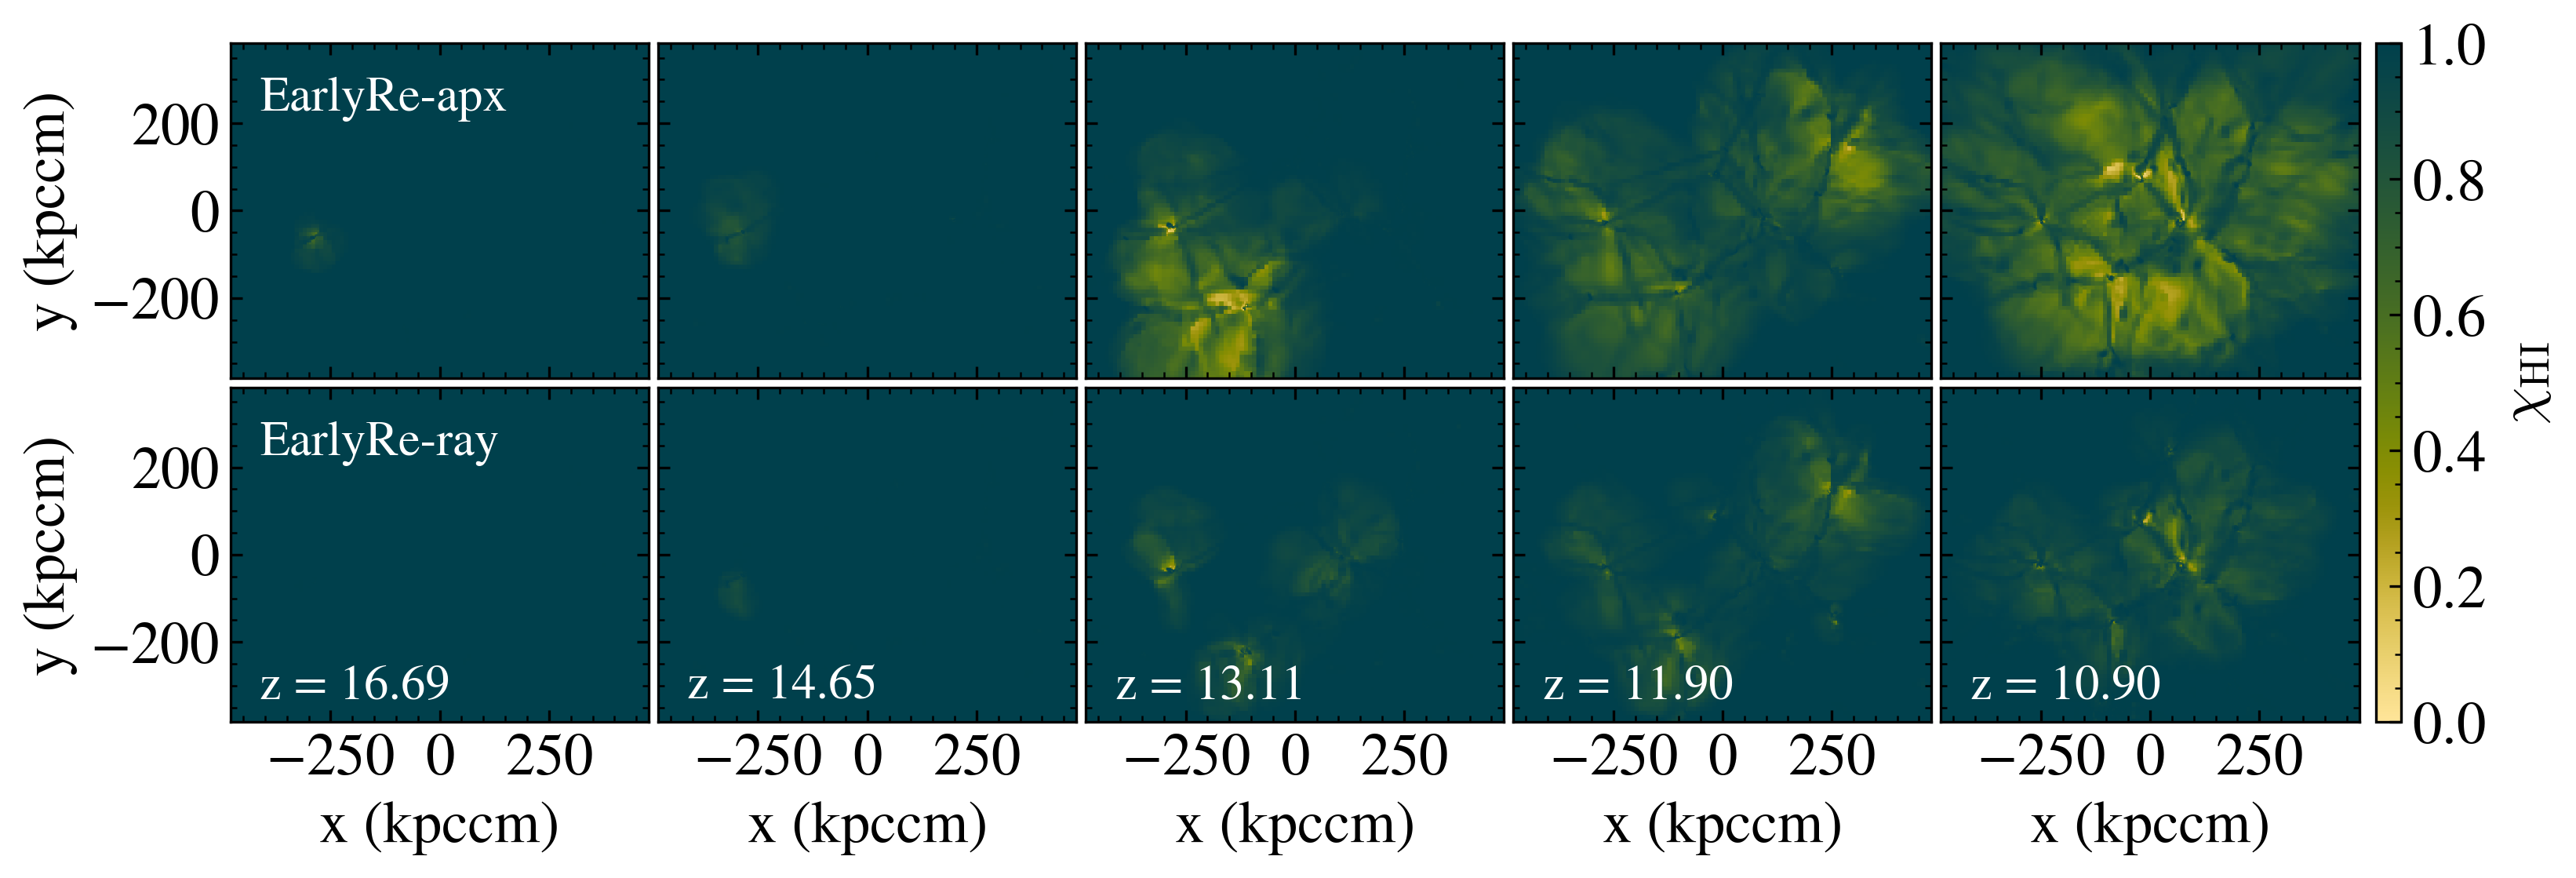
\includegraphics[width=\textwidth]{EarlyRe/neutralHfraction_comparison_multiple.png}
    \caption{The neutral hydrogen fraction in the whole refined region box between the \textit{EarlyRe-ray} and \textit{EarlyRe-apx} simulations.}
    \label{fig:neutralHfrac_map}
\end{figure*}

\begin{figure}
    \centering
    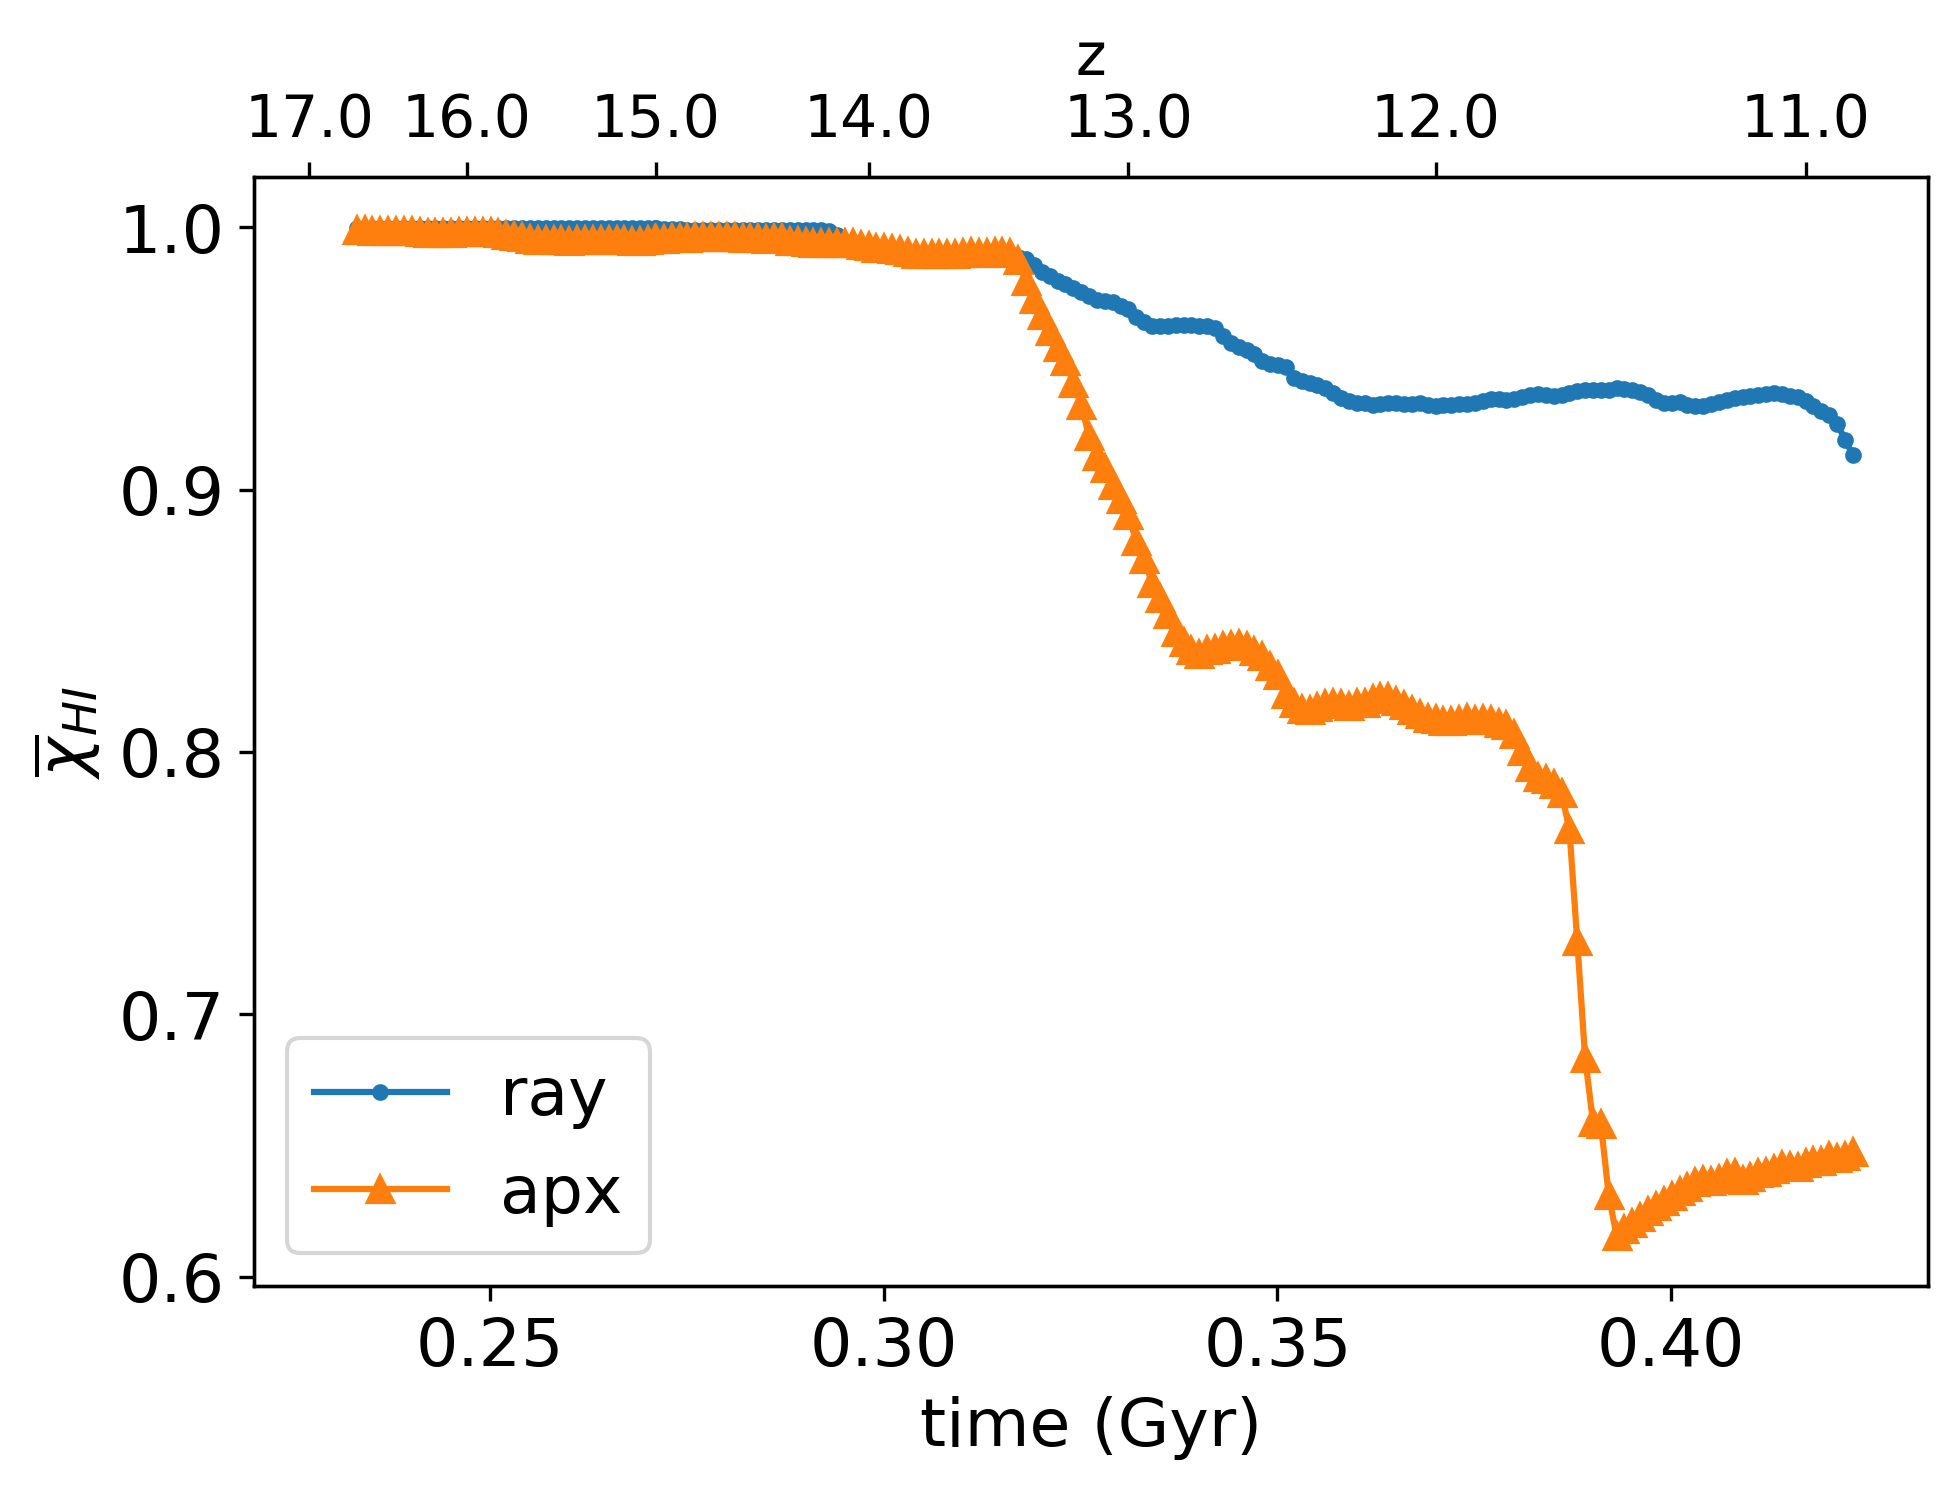
\includegraphics[width=0.95\columnwidth]{EarlyRe/neutralHfraction_evolution.png}
    \caption{The comparison between the volume-weighted average of the neutral hydrogen fraction as a function of time between the \textit{EarlyRe-ray} and the \textit{EarlyRe-apx} simulations.}
    \label{fig:neutralHfrac_evolution}
\end{figure}


\subsection{Investigation on late reionization period}
Include the analysis for the LateRe set

%\subsection{\textit{LateRe} simulation set}

%Section~\ref{sec:result_EarlyRe} establishes that the approximated model of molecular hydrogen self-shielding considerably alters the stellar mass outcome of cosmological simulation in the early epoch of reionization. In this section, we want to examine the applicability of this approximation in predicting the stellar mass at the late end of reionization ($z \approx 6 - 7)$, where the UV radiation is higher than at $z > 10$ by 1 dex \citep{Chardin+2018, Onorbe+2017}. Because evolving a whole cosmological simulation with ray-tracing treatment through the reionization period is rather expansive, to save computational time for the \textit{LateRe} set, we decide to run the two simulations \textit{LateRe-ray} and \textit{LateRe-apx} without ray-tracing from $z = 100$ to $z \approx 7.3$. At $z \approx 7.3$, we turn off the \textit{RadiativeTransferOpticallyThinH2} parameter to 0 for one of the simulations (the \textit{LateRe-ray}) and continue to run both of them to $z \approx 6.4$.

%Figure~\ref{fig:H2_frac_LateRe} displays the relationship between the $H_{2}$ fraction and the halo virial mass when we first turn off the \textit{RadiativeTransferOpticallyThinH2} to make the \textit{LateRe-ray} simulation (top panel) and at the last snapshot (bottom panel). The lines represent the average $H_{2}$ fraction of each halo mass bin. On the top panel, the two relations match each other well. This is expected because the optically thin approximation is just turned off for this snapshot, so there is not enough time for the ray-tracing model to result in any noticeable effects yet. After evolving the simulation to $z \approx 6.41$, the disparity becomes clearer. Similar to Figure~\ref{fig:H2_frac_EarlyRe}, the \textit{LateRe-ray} has a higher $H_{2}$ fraction than the \textit{LateRe-apx} in all mass bins, with the difference being larger in the smaller mass range. However, unlike Figure~\ref{fig:H2_frac_EarlyRe}, Figure~\ref{fig:H2_frac_LateRe} shows a bimodality in the $H_{2}$ fraction distribution in both simulations: a higher $H_{2}$ fraction of $\approx 10^{-4} - 10^{-1}$ region at the virial mass of $10^{7} - 5\times10^{8} M_\odot$ and a lower $H_{2}$ fraction of $\approx 10^{-10} - 10^{-8}$ region at the virial mass of $10^{6} - 5\times10^{7} M_\odot$. Because we do not see this behavior in the \textit{EarlyRe} set, it is likely that the high photoionization rate at the late Reionization causes this bimodality. At a higher mass, the halo's ability to be self-shielded increases due to its higher density; while the low-mass halos are more vulnerable for high LW radiation to photodissociate its molecular hydrogen content. Thus, in the case of lower-mass halos (lower region in the bottom plot), the choice of the self-shielding model becomes less influential (compared to Figure~\ref{fig:H2_frac_EarlyRe} of the \textit{EarlyRe} set) when determining the amount of the shielded hydrogen molecules. This is different than what we observe in the \textit{EarlyRe} set, where the $H_2$ fraction in the lower-mass halo is much higher when utilizing the ray-tracing treatment. Regarding the higher mass region of Figure~\ref{fig:H2_frac_LateRe}, the approximation causes the $H_{2}$ fraction to decrease by about 0.5 dex compared to the ray-tracing method.

%\begin{figure}
%    \centering
%    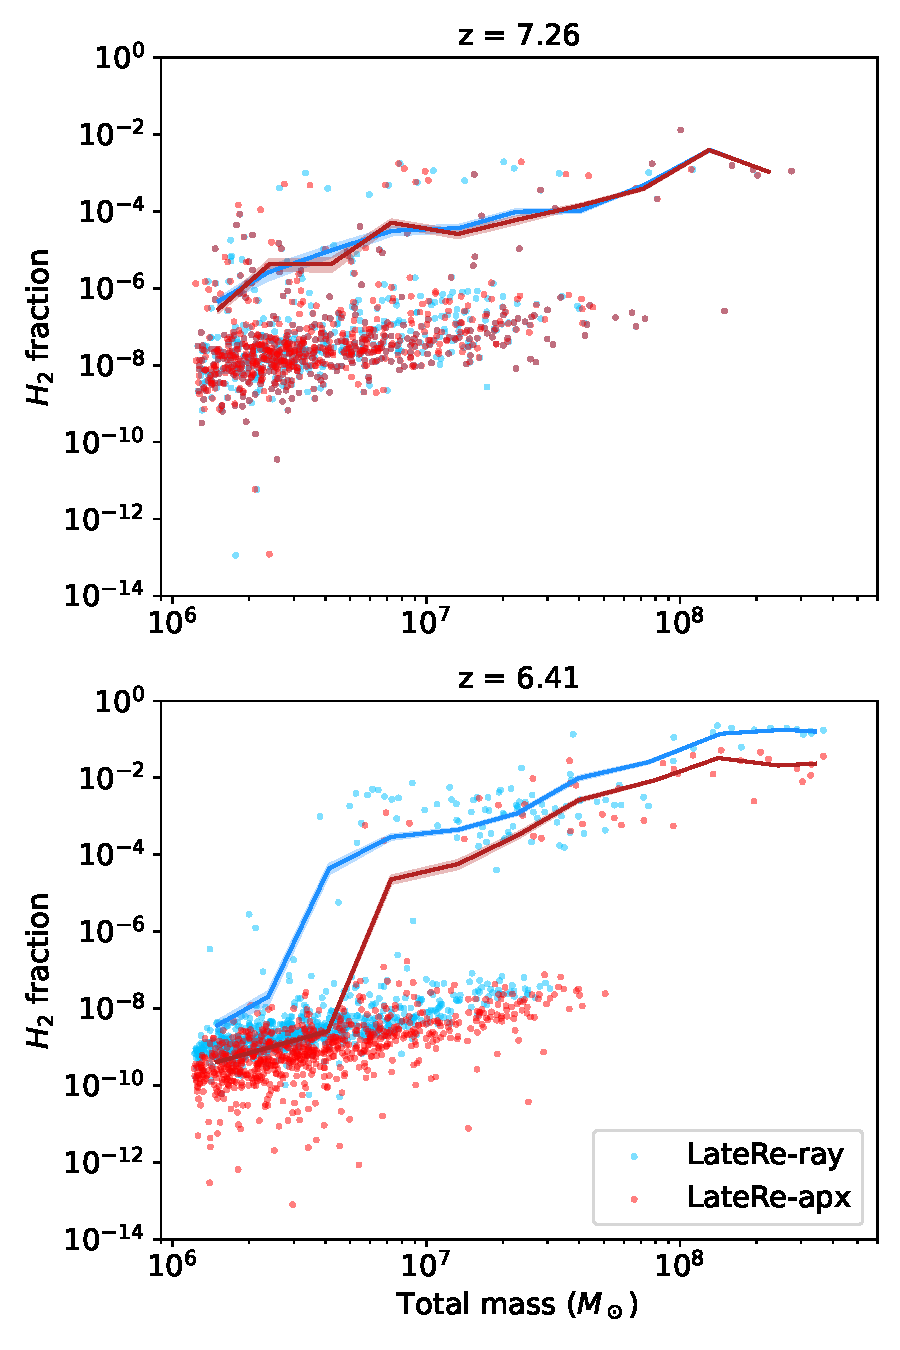
\includegraphics[width=0.9\columnwidth]{LateRe/h2_frac_distribution_LateRe.pdf}
%    \caption{The relationship between the $H_{2}$ fraction and the total mass at the first timestep and the last timestep of the \textit{LateRe} dataset.}
%    \label{fig:H2_frac_LateRe}
%\end{figure}

%Figure~\ref{fig:SFR_stellar_total_LateRe} shows the relationship between the SFR, stellar mass, and the halo virial mass of the two simulations in the \textit{LateRe} set. Unlike Figure~\ref{fig:SFR_stellar_total_EarlyRe}, at a later time of Reionization, the choice of the self-shielding models does not affect the stellar mass significantly. The distribution of stellar mass as a function of halo mass is similar between the ray-tracing treatment and the approximation treatment, even though the molecular hydrogen content is slightly higher in the \textit{LateRe-Ray} simulation in this mass range. Thus, the plot strengthens the fact that the self-shielding models do not significantly affect star formation activities at the late reionization epoch on a large scale. However, when we cross-match halos between the \textit{LateRe-ray} and the \textit{LateRe-apx} simulations, we notice some differences regarding their property evolution. Using the matching method detailed in Section~\ref{subsect:cross-matching_halos}, out of 14 \textit{LateRe-ray}'s halos and out of 15 \textit{LateRe-apx}'s halos that have non-zero stellar mass, we identify 12 matching halos between the two simulation sets. The other halos are located too far apart from each other to come from the same halos. 

%\begin{figure*}
%    \centering
%    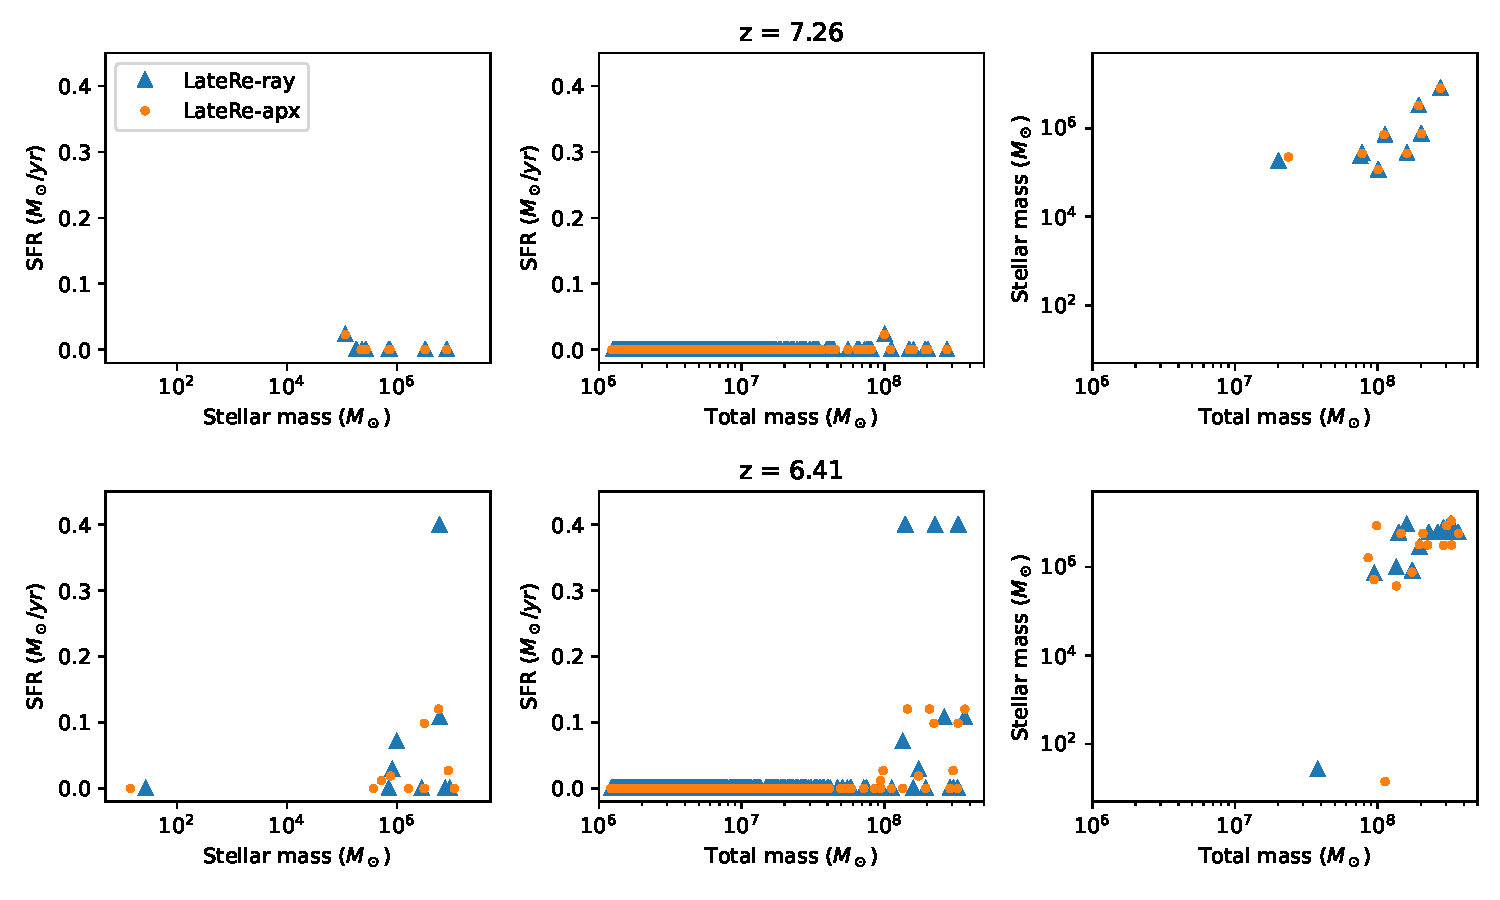
\includegraphics[width=0.9\textwidth]{LateRe/SFR_stellarmass_totalmass_LateRe.pdf}
%    \caption{The relationships between stellar mass, total mass, and star formation rate of all the halos in the first and in the last timestep}
%    \label{fig:SFR_stellar_total_LateRe}
%\end{figure*}

%CONSIDER TO REMOVE THIS, USE THE GAS PHASE PLOT INSTEAD
%\begin{figure}
%    \centering
%    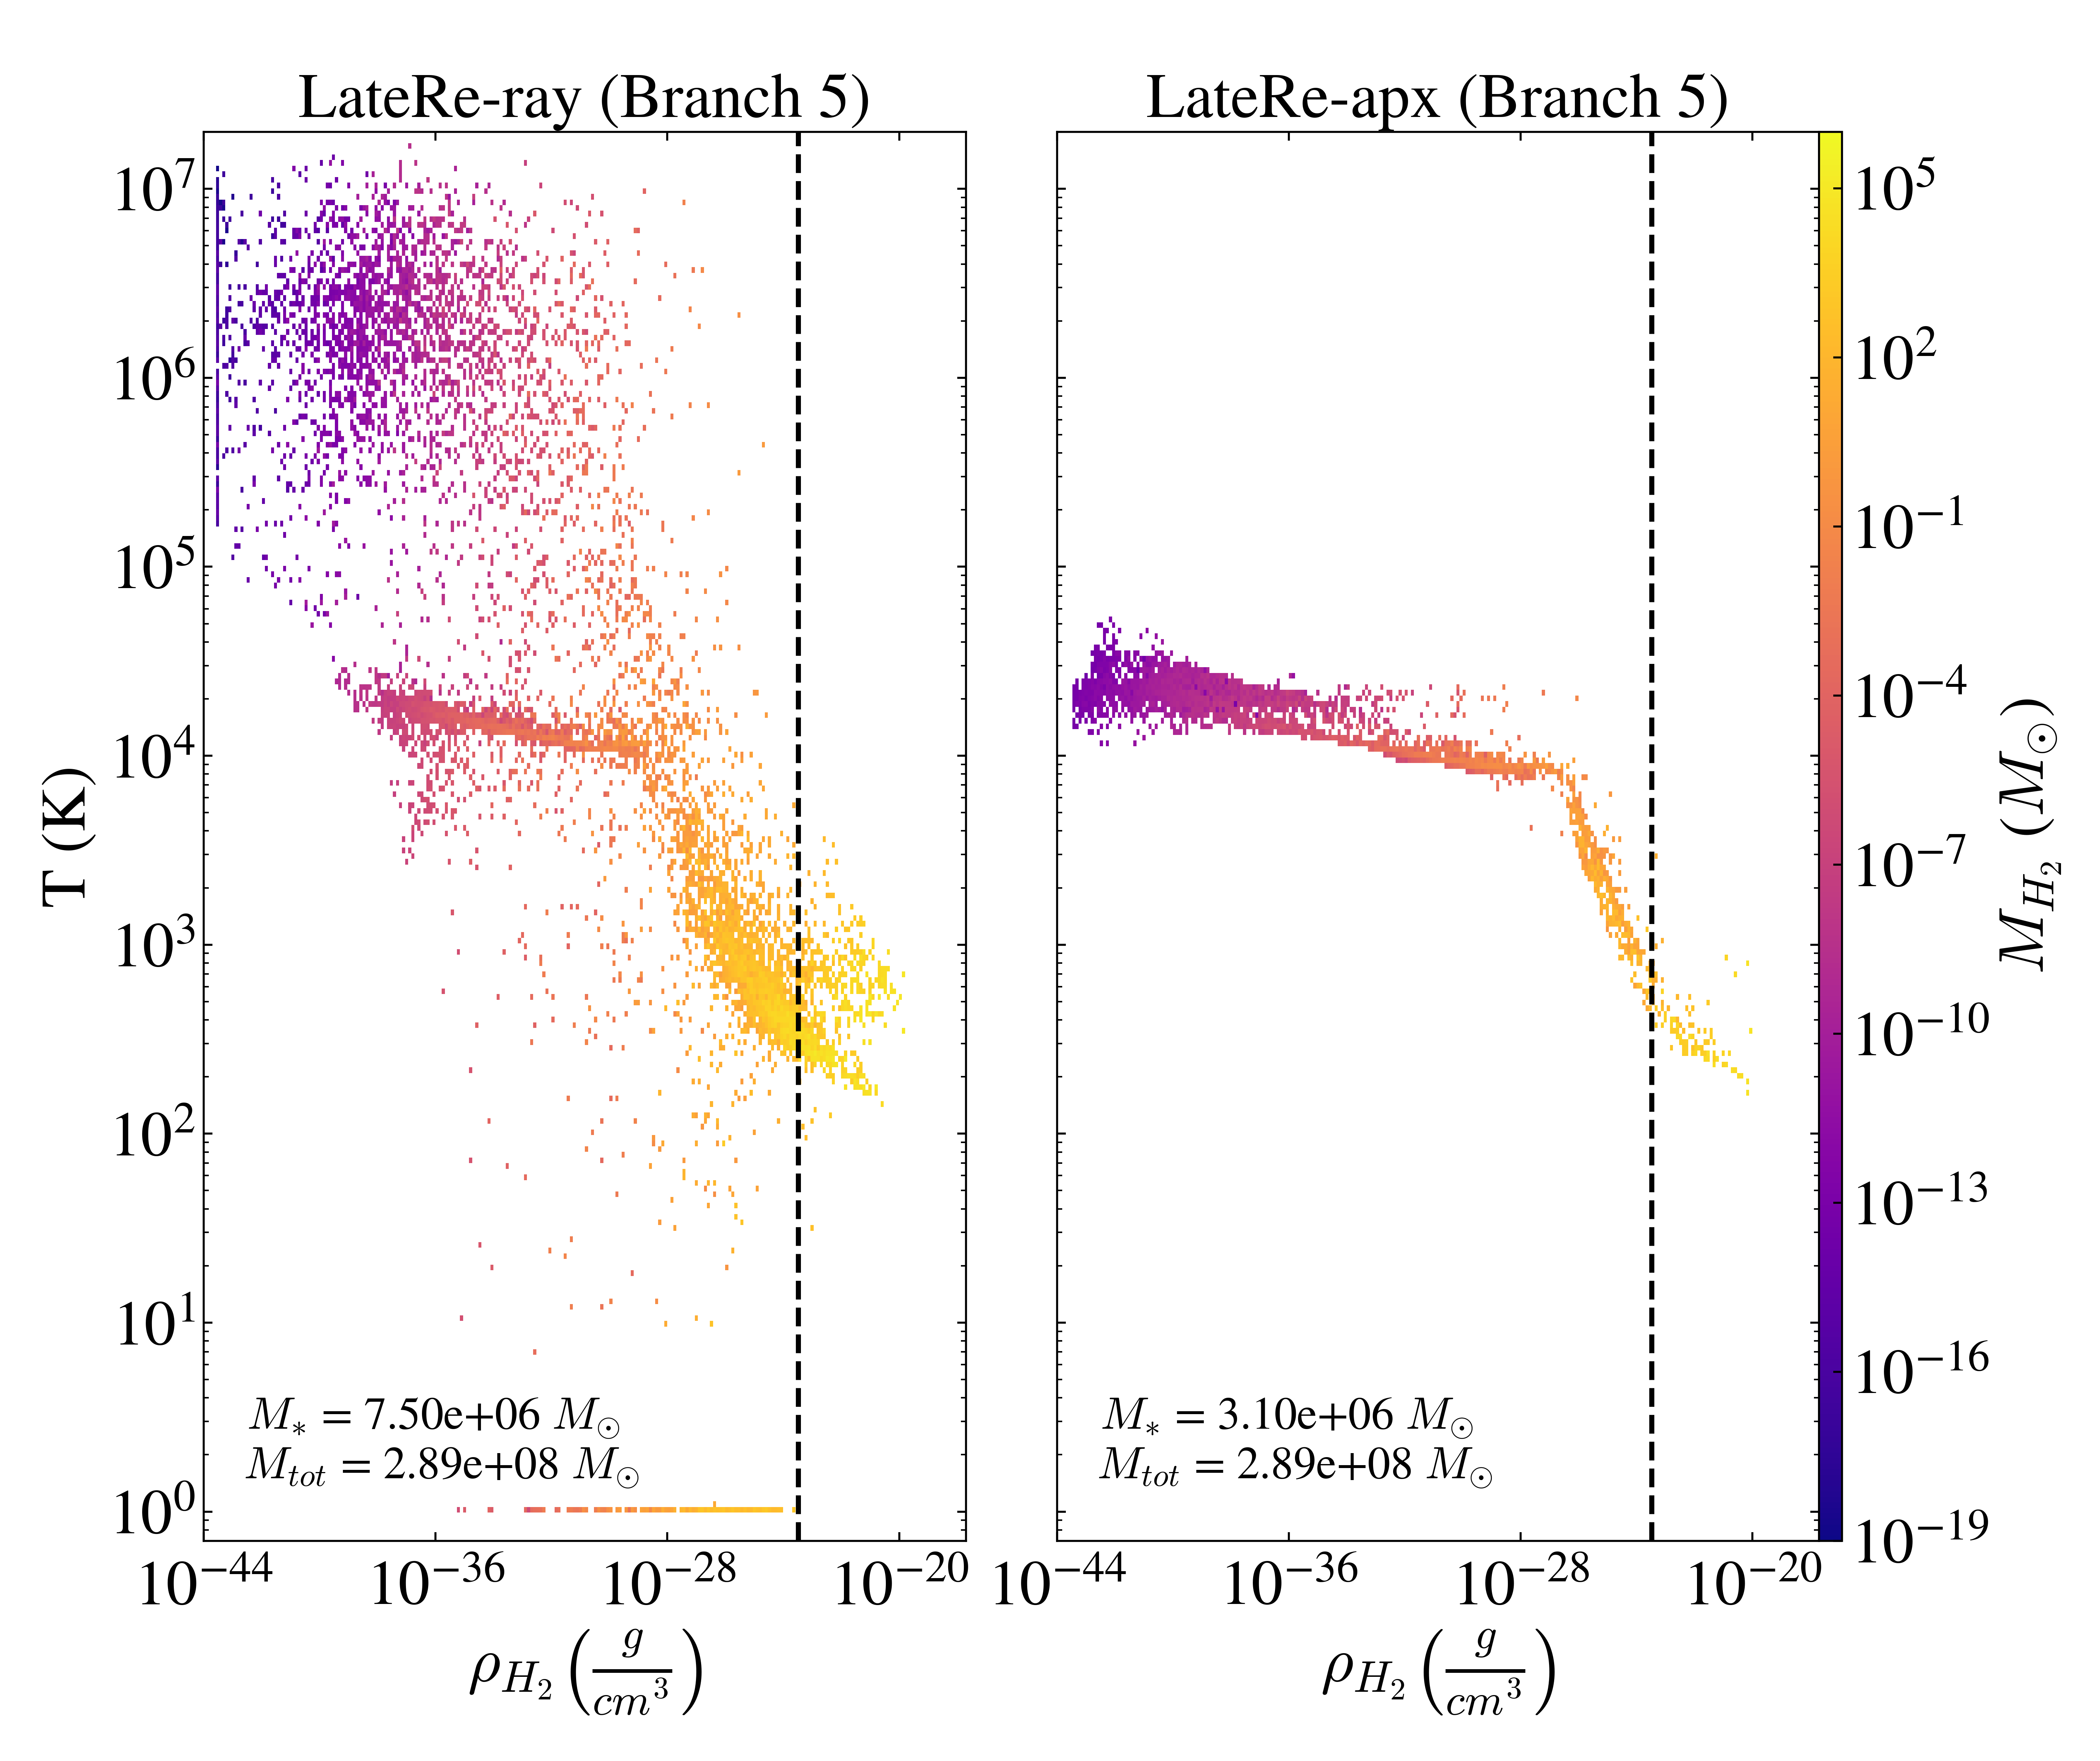
\includegraphics[width=\columnwidth]{LateRe/H2_phase_plot_comparison_branch_5-5_last_timestep_LateRe_tested.png}
%    \caption{The phase plot showing the temperature and density of molecular hydrogen gas in Halo Branch 5 (indexed by \texttt{consistent-tree} output) of \textit{LateRe-ray} and its counterpart in \textit{LateRe-apx}. The black dashed line represents the star formation density threshold $n_{H,thres} = 1 cm^{-3}$.}
%    \label{fig:H2_phase_plot_Branch-5_LateRe}
%\end{figure}

%Figure~\ref{fig:example_2_halos_LateRe} shows the evolution in gas mass fraction, $H_{2}$ fraction, stellar mass, and star formation in two of the twelve cross-matched halos. As pointed out in Figure~\ref{fig:H2_frac_LateRe}, in both halos, the \textit{LateRe-ray} version shields the molecular hydrogen better. However, the relative differences in stellar mass, gas mass fraction, and star formation rate are more random, even though they do change. For example, for the halo in the top panel, the \textit{LateRe-apx} halo gains about 1.2 times more stellar mass than the \textit{LateRe-ray} halo. On the other hand, for the halo at the bottom panel, the ray-tracing treatment brings about a 2.5 times increase in stellar mass in the last snapshot. Their star formation history also differs. For instance, the \textit{LateRe-apx}'s halo in the top panel experiences a quick burst of star formation while we do not see that in the \textit{LateRe-ray} one. For brevity, we do not show the plots of other cross-matched halos here, but given the small sample size of only 12 halos, we detect no patterns regarding the differences between the two halos in terms of stellar mass or star formation history. Regardless, it is still important to note that the amount of molecular hydrogen changes significantly between the two sets.

%\begin{figure}
%    \gridline{\fig{LateRe/Branch_3_evolution_LateRe.pdf}{0.9\columnwidth}{}}
%    \gridline{\fig{LateRe/Branch_5_evolution_LateRe.pdf}{0.9\columnwidth}{}}
%    \caption{The gas mass fraction, the stellar mass, the $H_{2}$ fraction, and the star formation history of the same halo in \textit{LateRe-ray} and in \textit{LateRe-apx}. Two halos at different total mass ranges are given as an example.}
%    \label{fig:example_2_halos_LateRe}
%\end{figure}

\section{Conclusions and Discussions}
Maybe mention that the Renaissance Simulation (and maybe others) doesn't implement self-shielding, so can affect the results.

The strong radiation in late reionization destroys H2 in both \textit{ray} and \textit{apx} sets. This is reflected by the fact that the separation between the \textit{ray} and the \textit{apx} is not as prominent as in the EarlyRe set. In the EarlyRe set, the radiation is still weak, thus it only affects the non-shielding version. The halos of \textit{ray} version are shielded with this weak radiation, but not with the strong radiation as in LateRe.  

\textbf{Remember to use bullet points for each main result and specifically state the figure associated with each main result.}

%% IMPORTANT! The old "\acknowledgment" command has be depreciated. It was
%% not robust enough to handle our new dual anonymous review requirements and
%% thus been replaced with the acknowledgment environment. If you try to 
%% compile with \acknowledgment you will get an error print to the screen
%% and in the compiled pdf.
%% 
%% Also note that the akcnowlodgment environment does not support long amounts of text. If you have a lot of people and institutions to acknowledge, do not use this command. Instead, create a new \section{Acknowledgments}.
\begin{acknowledgments}
Acknowledgement: ---
\end{acknowledgments}

%% To help institutions obtain information on the effectiveness of their 
%% telescopes the AAS Journals has created a group of keywords for telescope 
%% facilities.
%
%% Following the acknowledgments section, use the following syntax and the
%% \facility{} or \facilities{} macros to list the keywords of facilities used 
%% in the research for the paper.  Each keyword is check against the master 
%% list during copy editing.  Individual instruments can be provided in 
%% parentheses, after the keyword, but they are not verified.

\vspace{5mm}
%\facilities{HST(STIS), Swift(XRT and UVOT), AAVSO, CTIO:1.3m}

%% Similar to \facility{}, there is the optional \software command to allow 
%% authors a place to specify which programs were used during the creation of 
%% the manuscript. Authors should list each code and include either a
%% citation or url to the code inside ()s when available.

%\software{astropy, Cloudy, Source Extractor}

%% Appendix material should be preceded with a single \appendix command.
%% There should be a \section command for each appendix. Mark appendix
%% subsections with the same markup you use in the main body of the paper.

%% Each Appendix (indicated with \section) will be lettered A, B, C, etc.
%% The equation counter will reset when it encounters the \appendix
%% command and will number appendix equations (A1), (A2), etc. The
%% Figure and Table counter will not reset.


%% For this sample we use BibTeX plus aasjournals.bst to generate the
%% the bibliography. The sample631.bib file was populated from ADS. To
%% get the citations to show in the compiled file do the following:
%%
%% pdflatex sample631.tex
%% bibtext sample631
%% pdflatex sample631.tex
%% pdflatex sample631.tex

\bibliography{sample631}{}
\bibliographystyle{aasjournal}

%% This command is needed to show the entire author+affiliation list when
%% the collaboration and author truncation commands are used.  It has to
%% go at the end of the manuscript.
%\allauthors

%% Include this line if you are using the \added, \replaced, \deleted
%% commands to see a summary list of all changes at the end of the article.
%\listofchanges

\end{document}

% End of file `sample631.tex'.
